\clearpage
\section*{Appendix C: Sheets of All Components}
\addcontentsline{toc}{section}{Appendix C: Sheets of All Components}

In each row, the first column shows the time course of $S$, the second column the PSD, and the third column the mixing weights, or the map of the corresponding column of $A$. Blue means kept and red means removed. In the real-data maps, the nose points upward and the left side of the person is on the left of the image. The polar coordinates of the electrode file were used so that A1 and A2 are not placed inside the temporal electrodes of the image. The color of the points shows the true value of the weight, and the interpolation outside the convex hull was not extrapolated.

The IC numbers cannot be matched directly between the two simulation decompositions. The scale and the sign of the map of each component must be read with the color bar of that same map. For the simulation data, the weight column is a bar plot, so that the mixing pattern can be examined without an additional geometric assumption.

\begin{figure}[p]
\centering
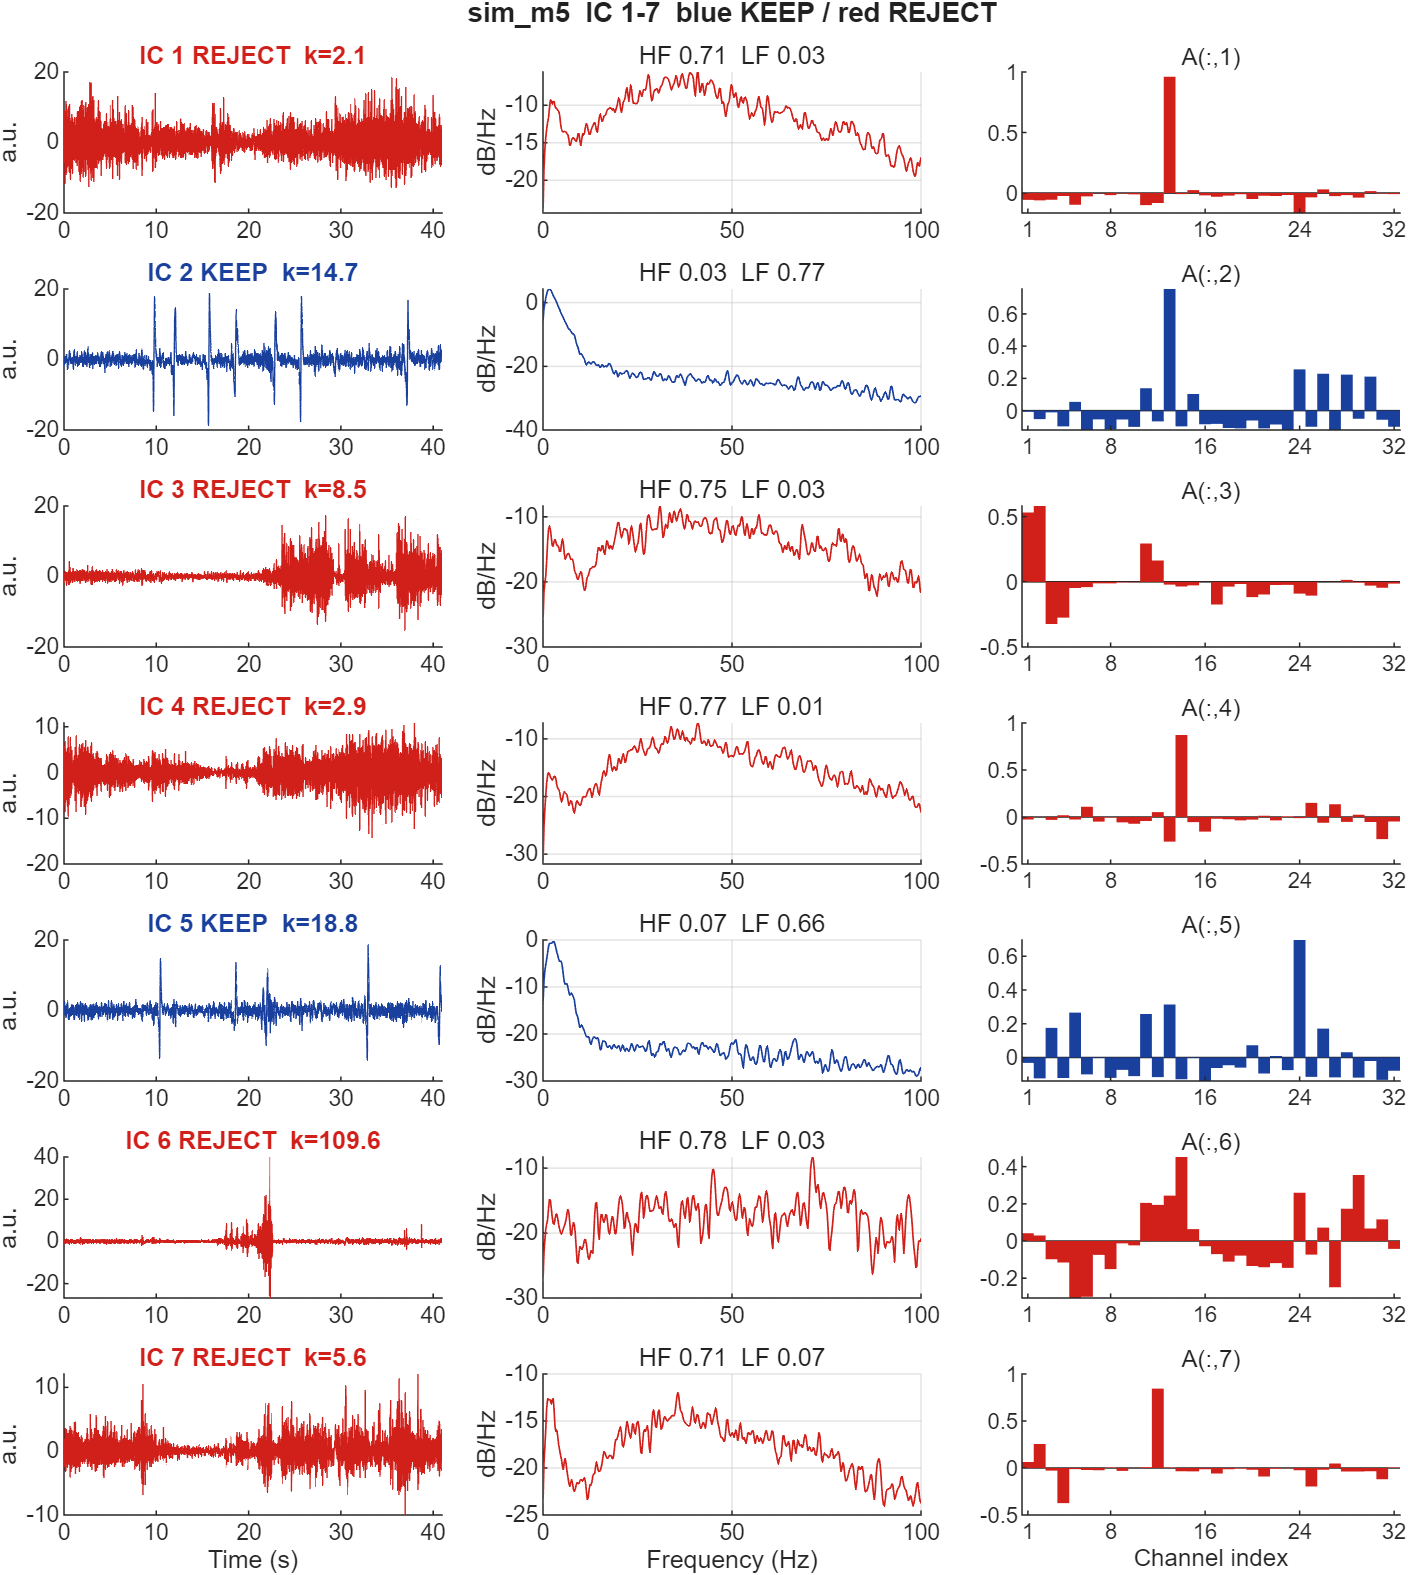
\includegraphics[height=0.80\textheight,width=0.95\textwidth,keepaspectratio]{fig16_sim_m5db_ic01_to_ic07.png}
\caption{Time course, PSD and mixing pattern of components components 1 to 7 in the $-5$~dB simulation.}
\label{fig:app16}
\end{figure}
\begin{figure}[p]
\centering
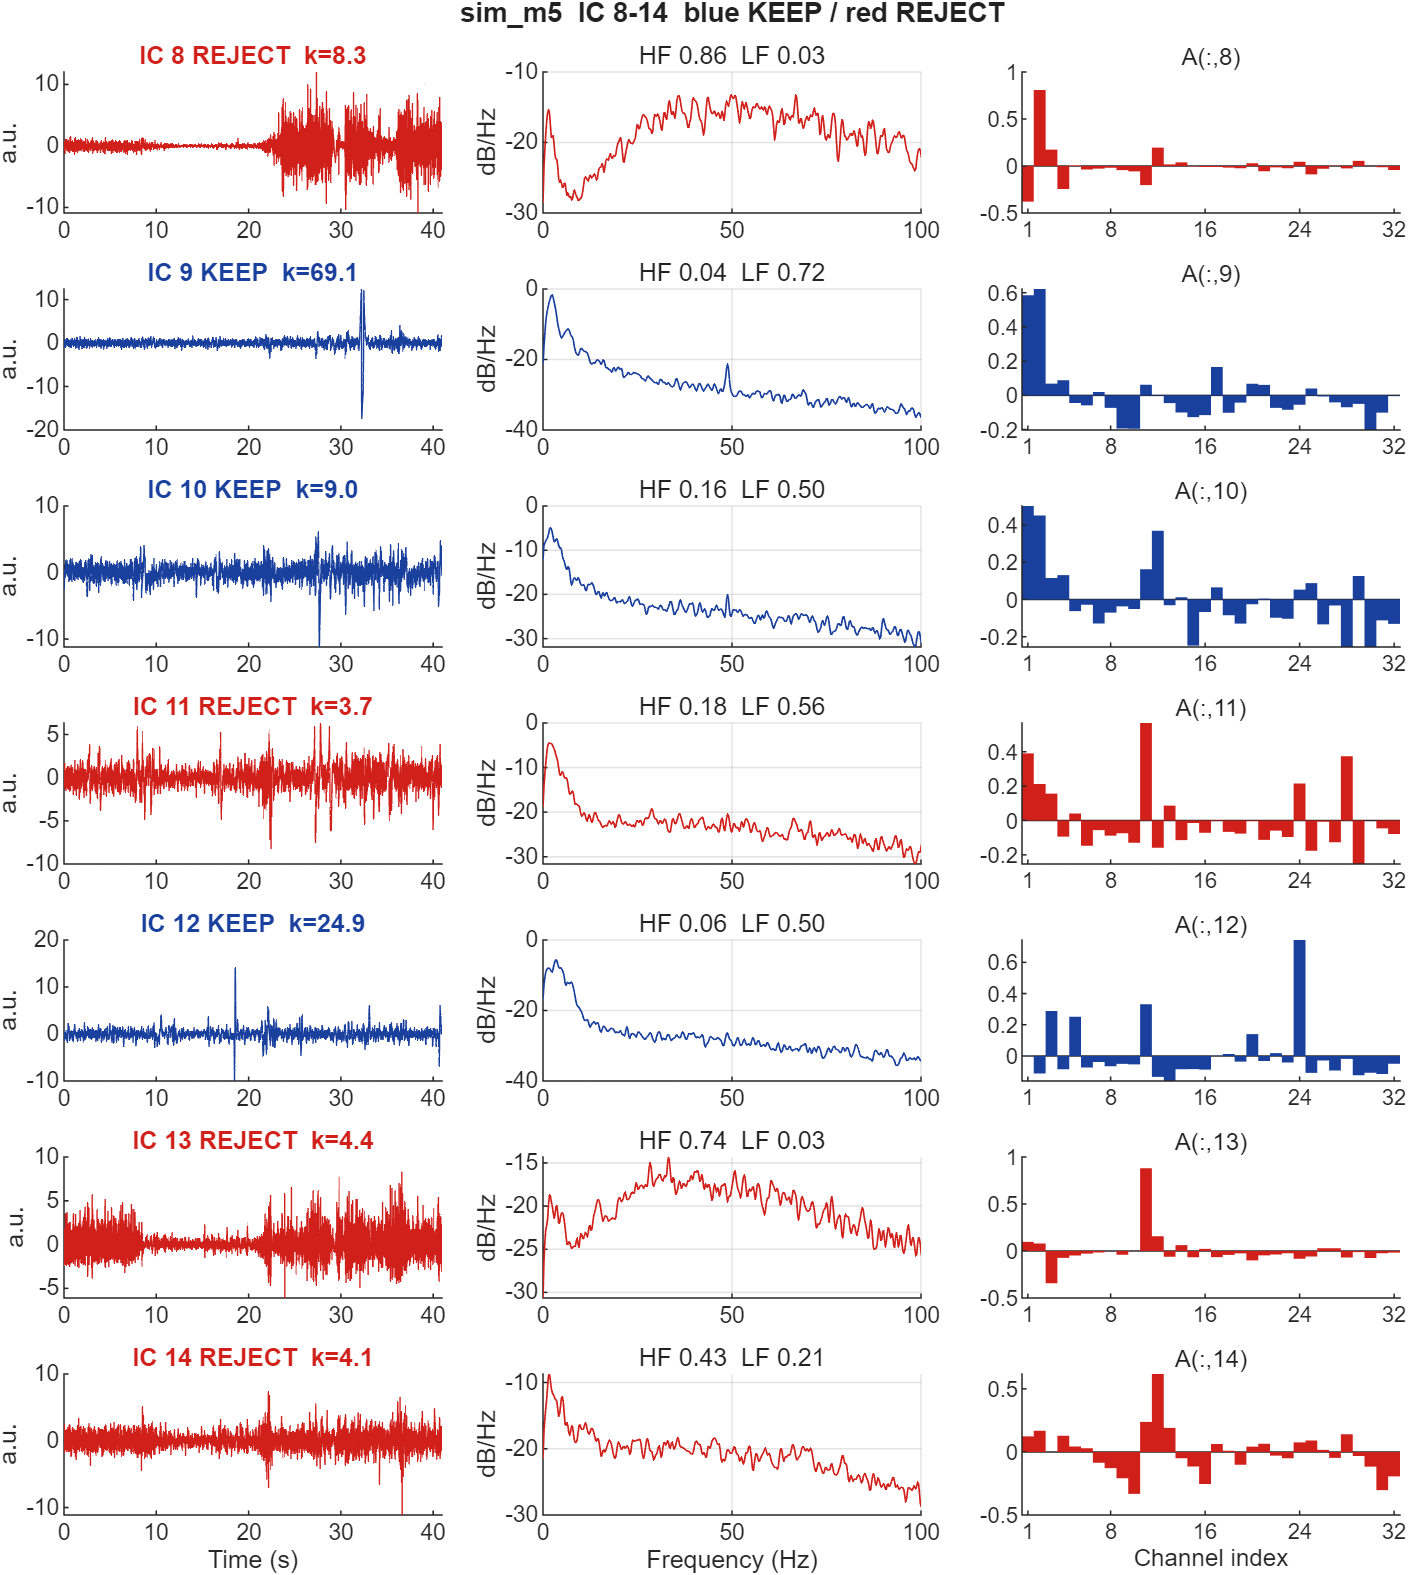
\includegraphics[height=0.80\textheight,width=0.95\textwidth,keepaspectratio]{fig17_sim_m5db_ic08_to_ic14.png}
\caption{Time course, PSD and mixing pattern of components components 8 to 14 in the $-5$~dB simulation.}
\label{fig:app17}
\end{figure}
\begin{figure}[p]
\centering
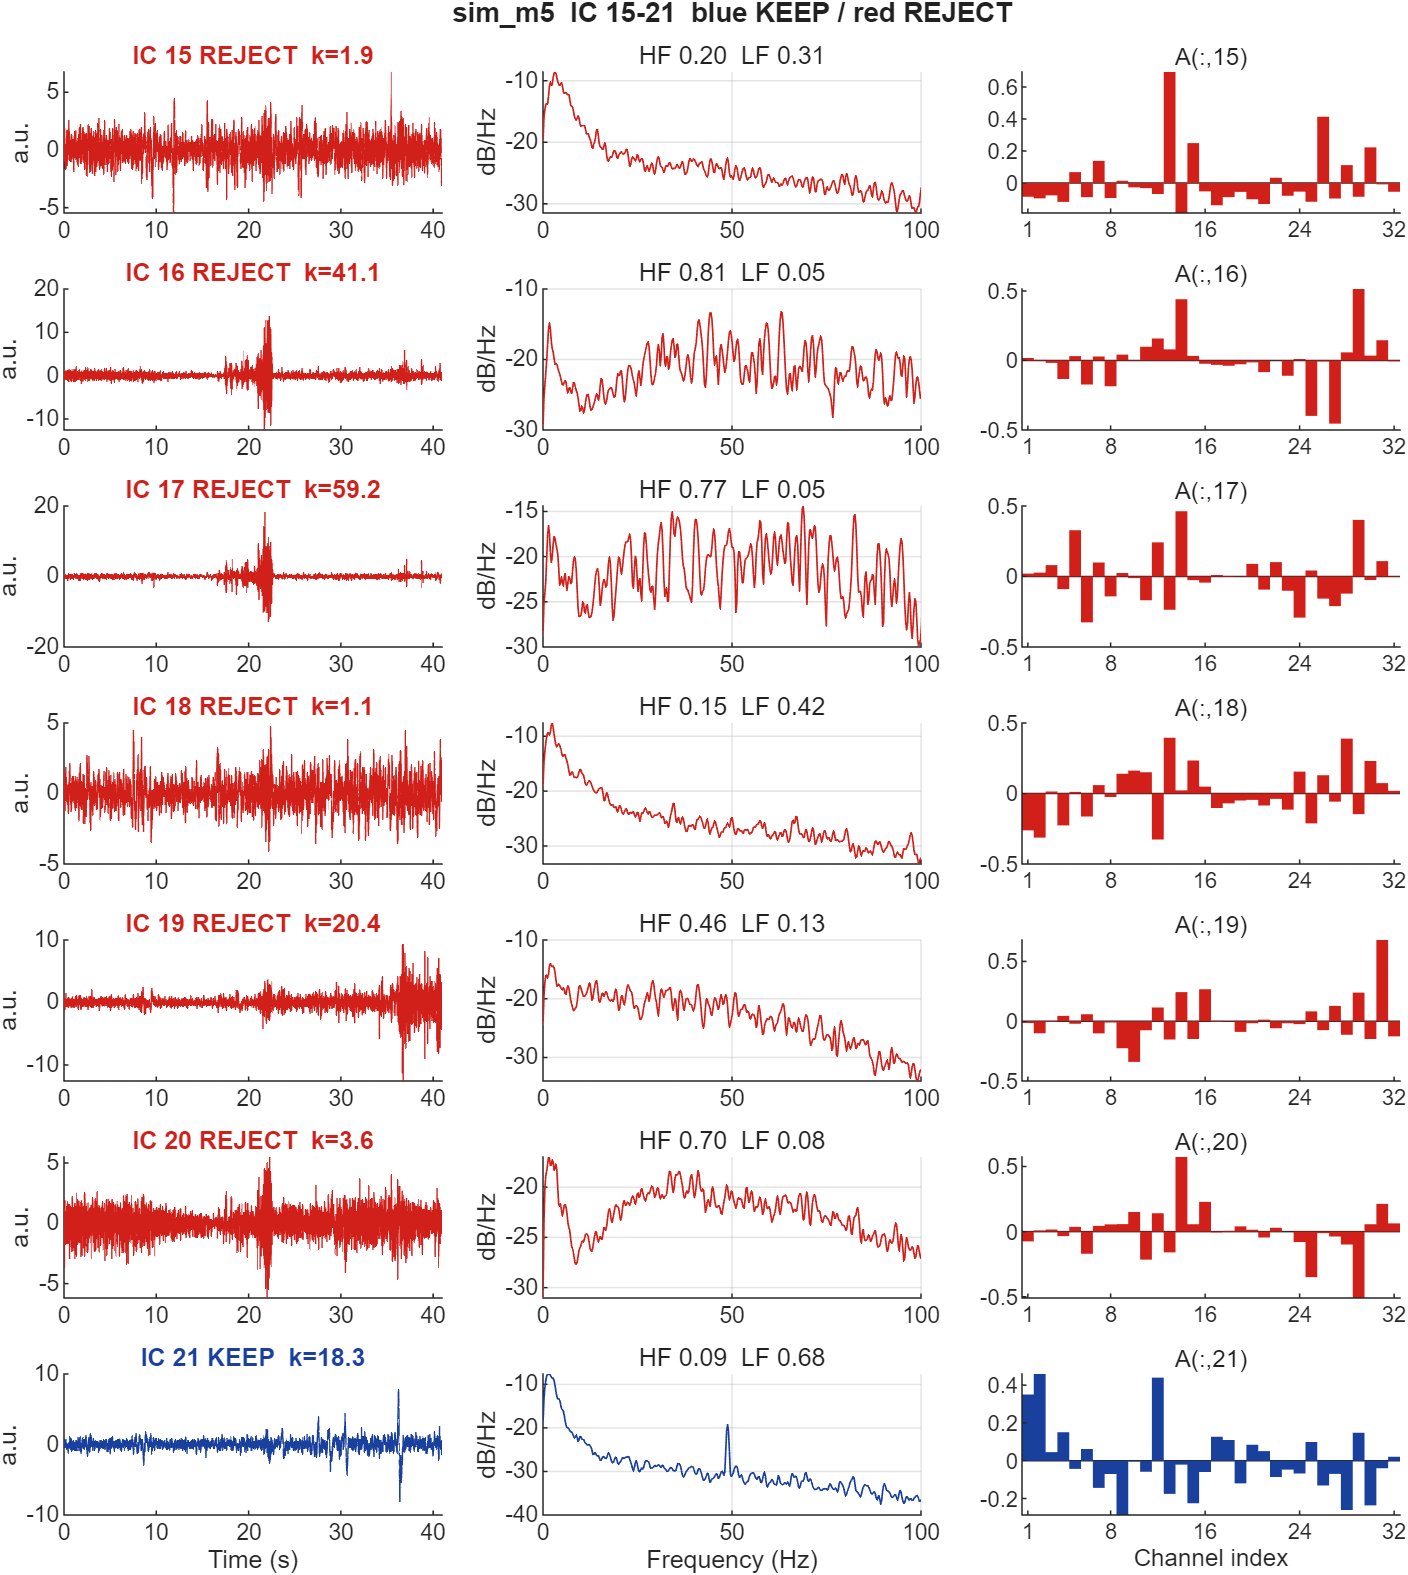
\includegraphics[height=0.80\textheight,width=0.95\textwidth,keepaspectratio]{fig18_sim_m5db_ic15_to_ic21.png}
\caption{Time course, PSD and mixing pattern of components components 15 to 21 in the $-5$~dB simulation.}
\label{fig:app18}
\end{figure}
\begin{figure}[p]
\centering
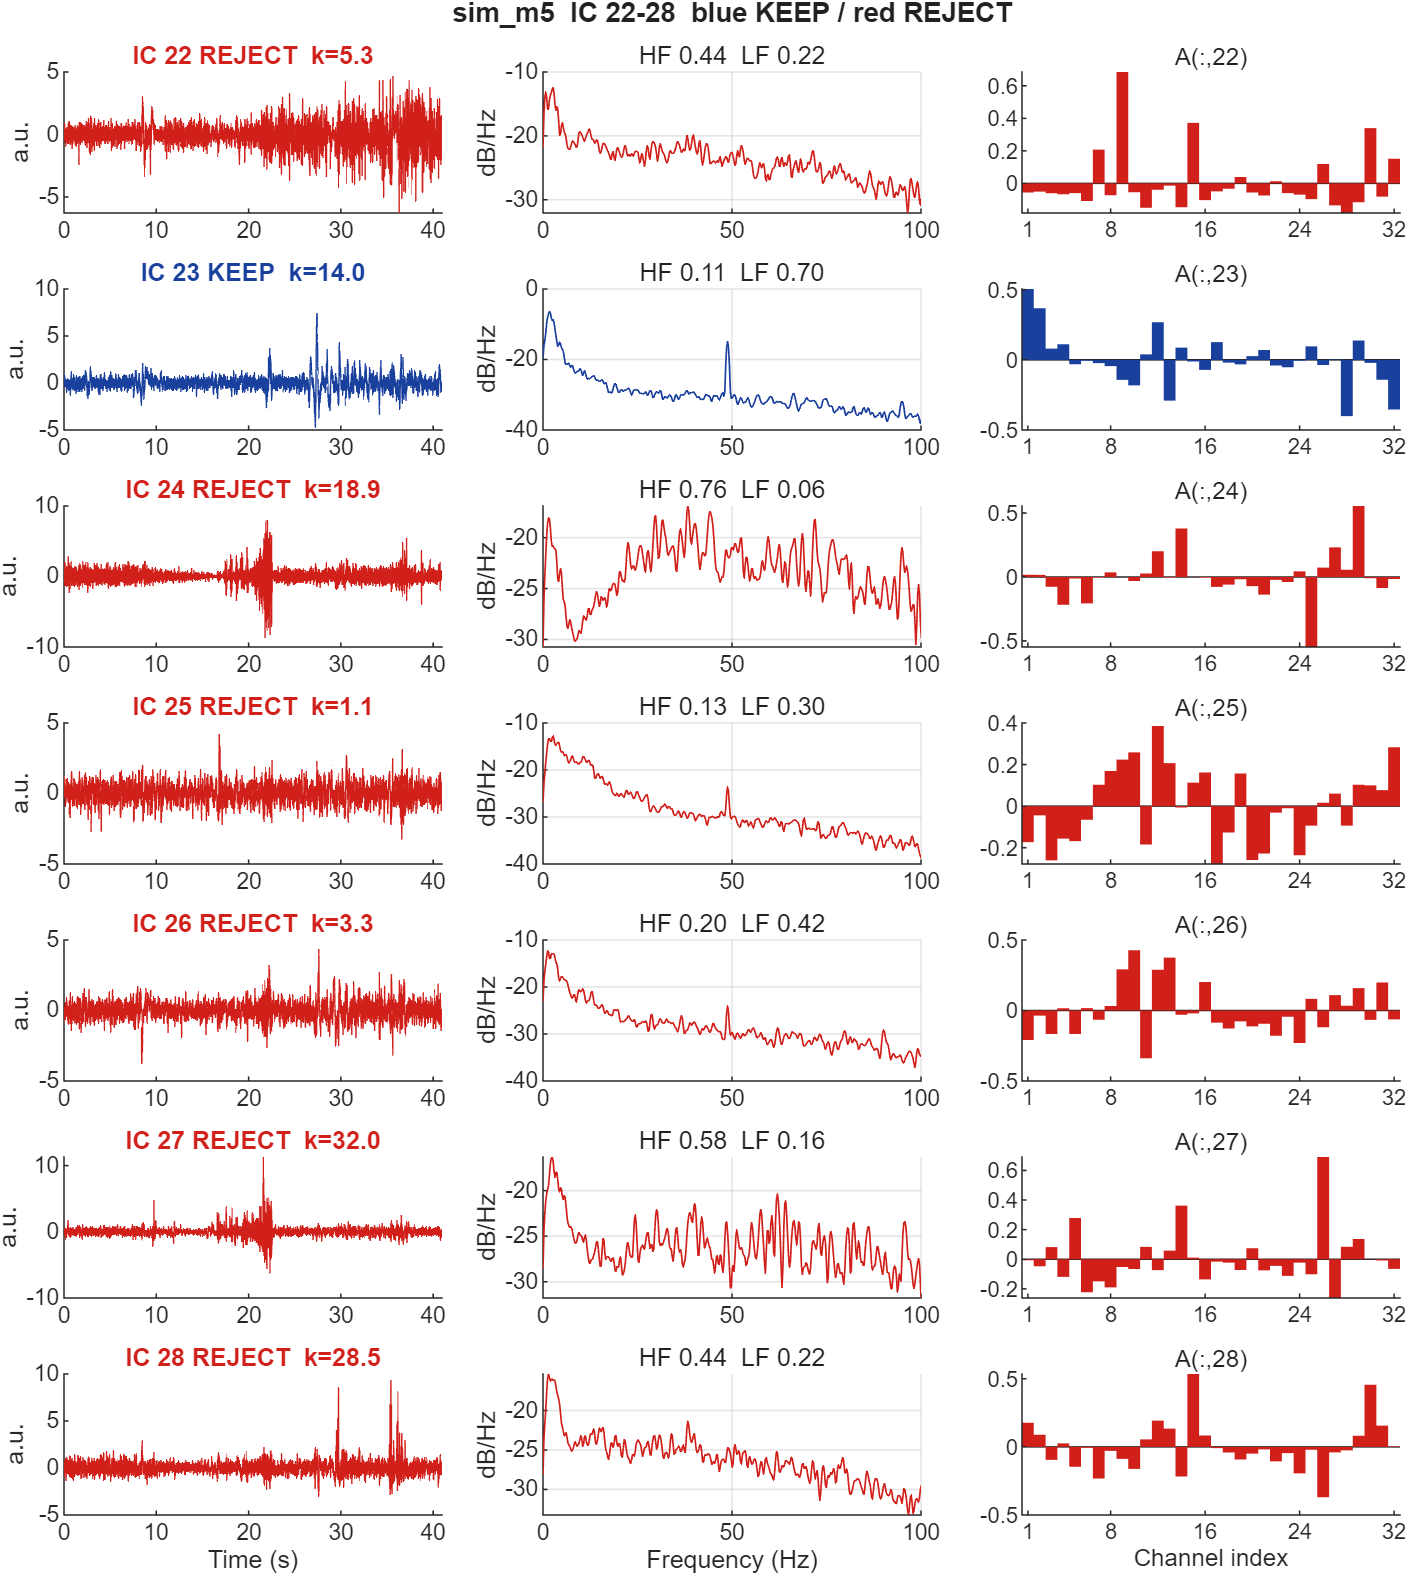
\includegraphics[height=0.80\textheight,width=0.95\textwidth,keepaspectratio]{fig19_sim_m5db_ic22_to_ic28.png}
\caption{Time course, PSD and mixing pattern of components components 22 to 28 in the $-5$~dB simulation.}
\label{fig:app19}
\end{figure}
\begin{figure}[p]
\centering
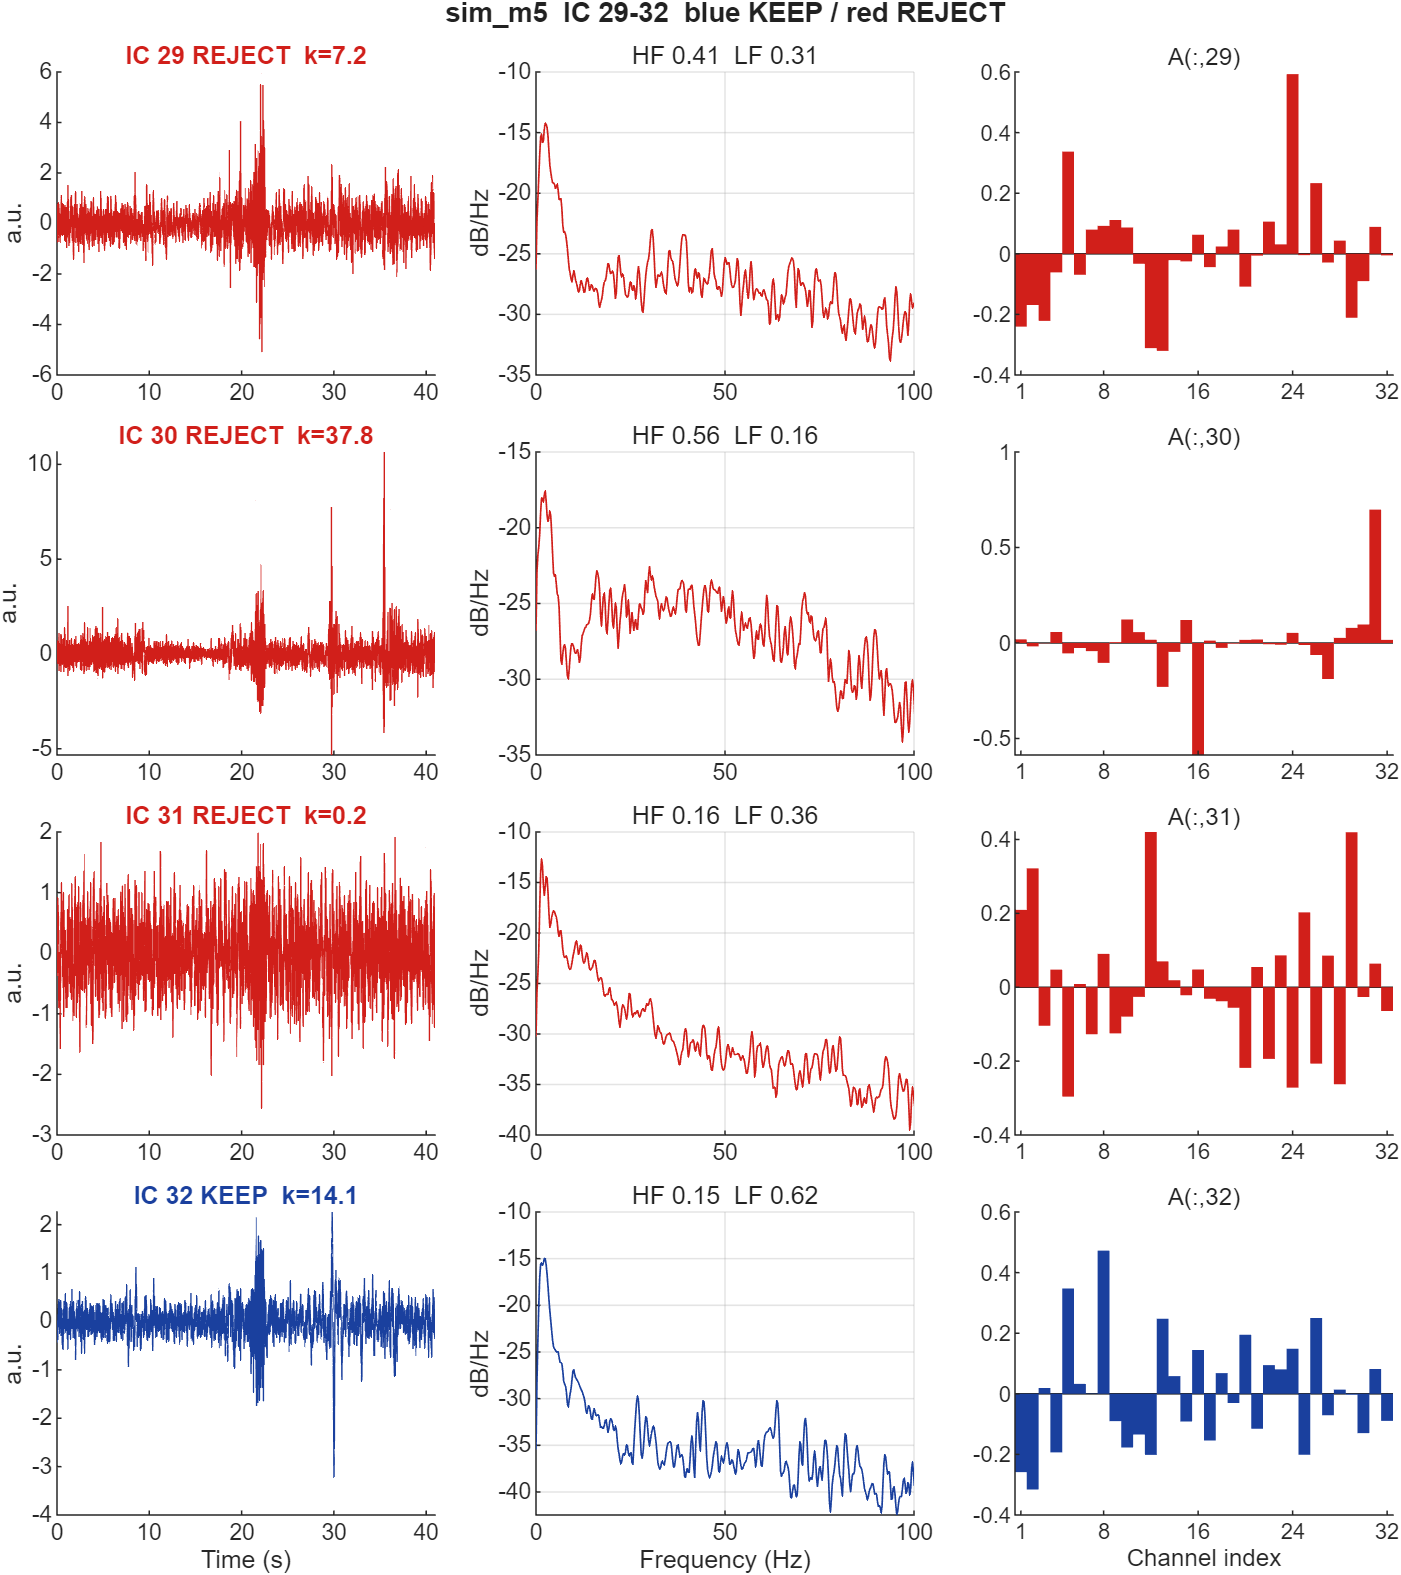
\includegraphics[height=0.80\textheight,width=0.95\textwidth,keepaspectratio]{fig20_sim_m5db_ic29_to_ic32.png}
\caption{Time course, PSD and mixing pattern of components components 29 to 32 in the $-5$~dB simulation.}
\label{fig:app20}
\end{figure}
\begin{figure}[p]
\centering
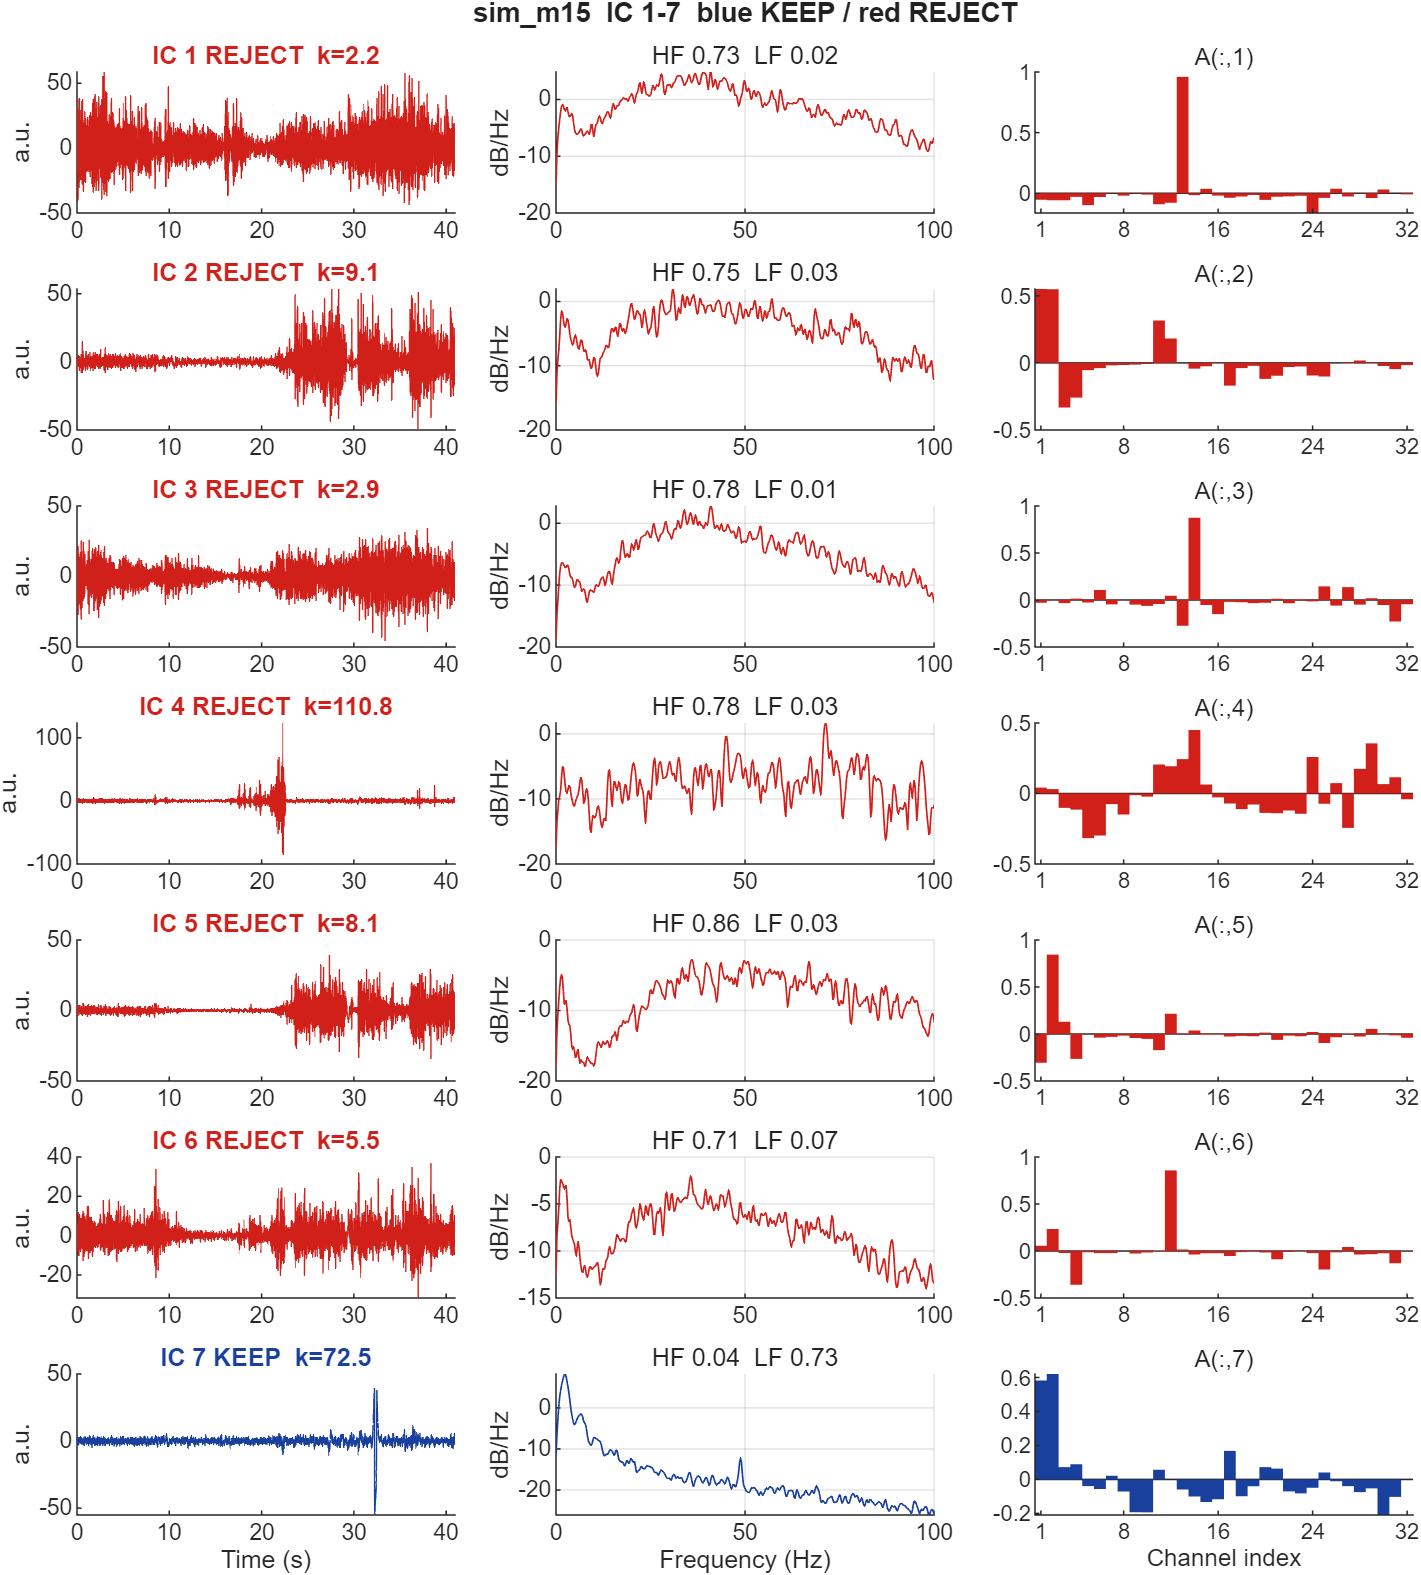
\includegraphics[height=0.80\textheight,width=0.95\textwidth,keepaspectratio]{fig21_sim_m15db_ic01_to_ic07.png}
\caption{Time course, PSD and mixing pattern of components components 1 to 7 in the $-15$~dB simulation.}
\label{fig:app21}
\end{figure}
\begin{figure}[p]
\centering
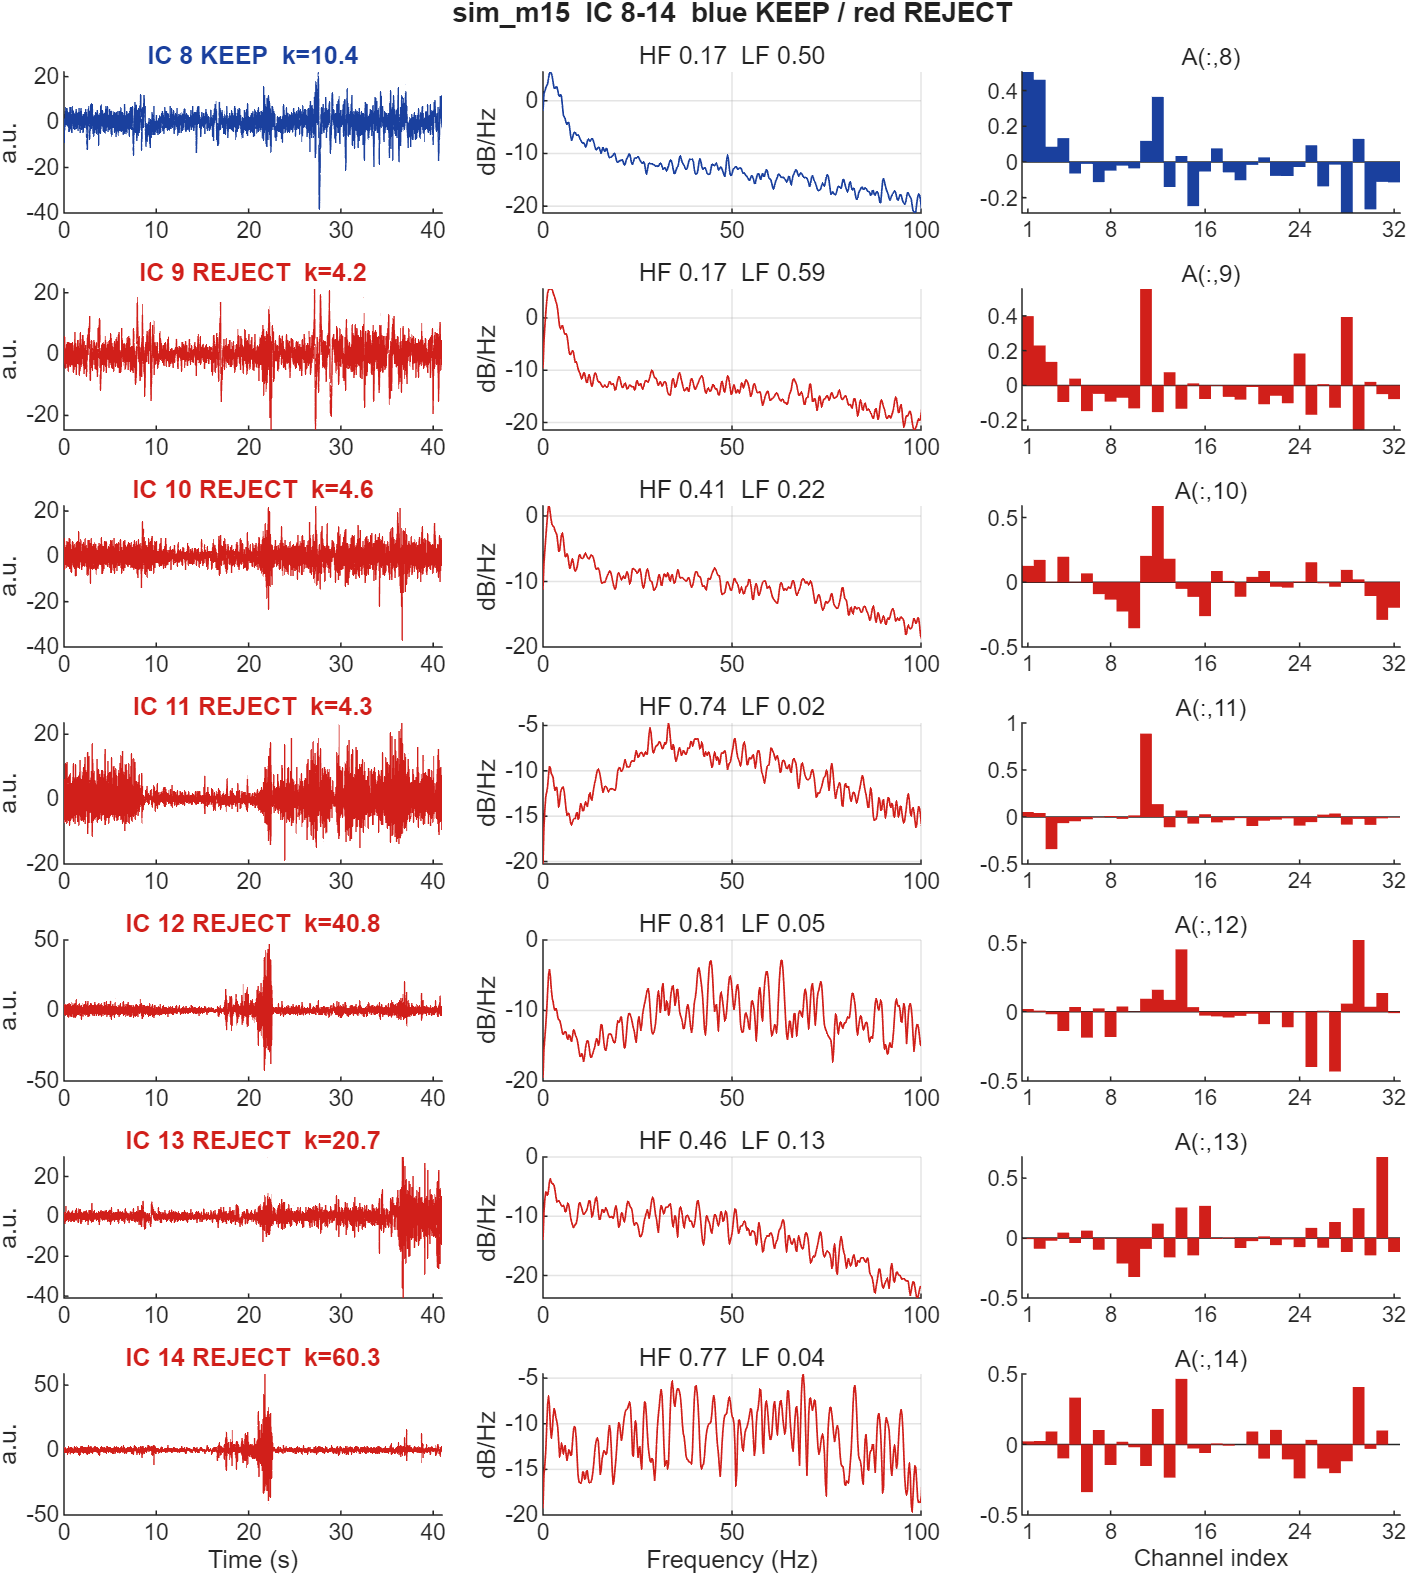
\includegraphics[height=0.80\textheight,width=0.95\textwidth,keepaspectratio]{fig22_sim_m15db_ic08_to_ic14.png}
\caption{Time course, PSD and mixing pattern of components components 8 to 14 in the $-15$~dB simulation.}
\label{fig:app22}
\end{figure}
\begin{figure}[p]
\centering
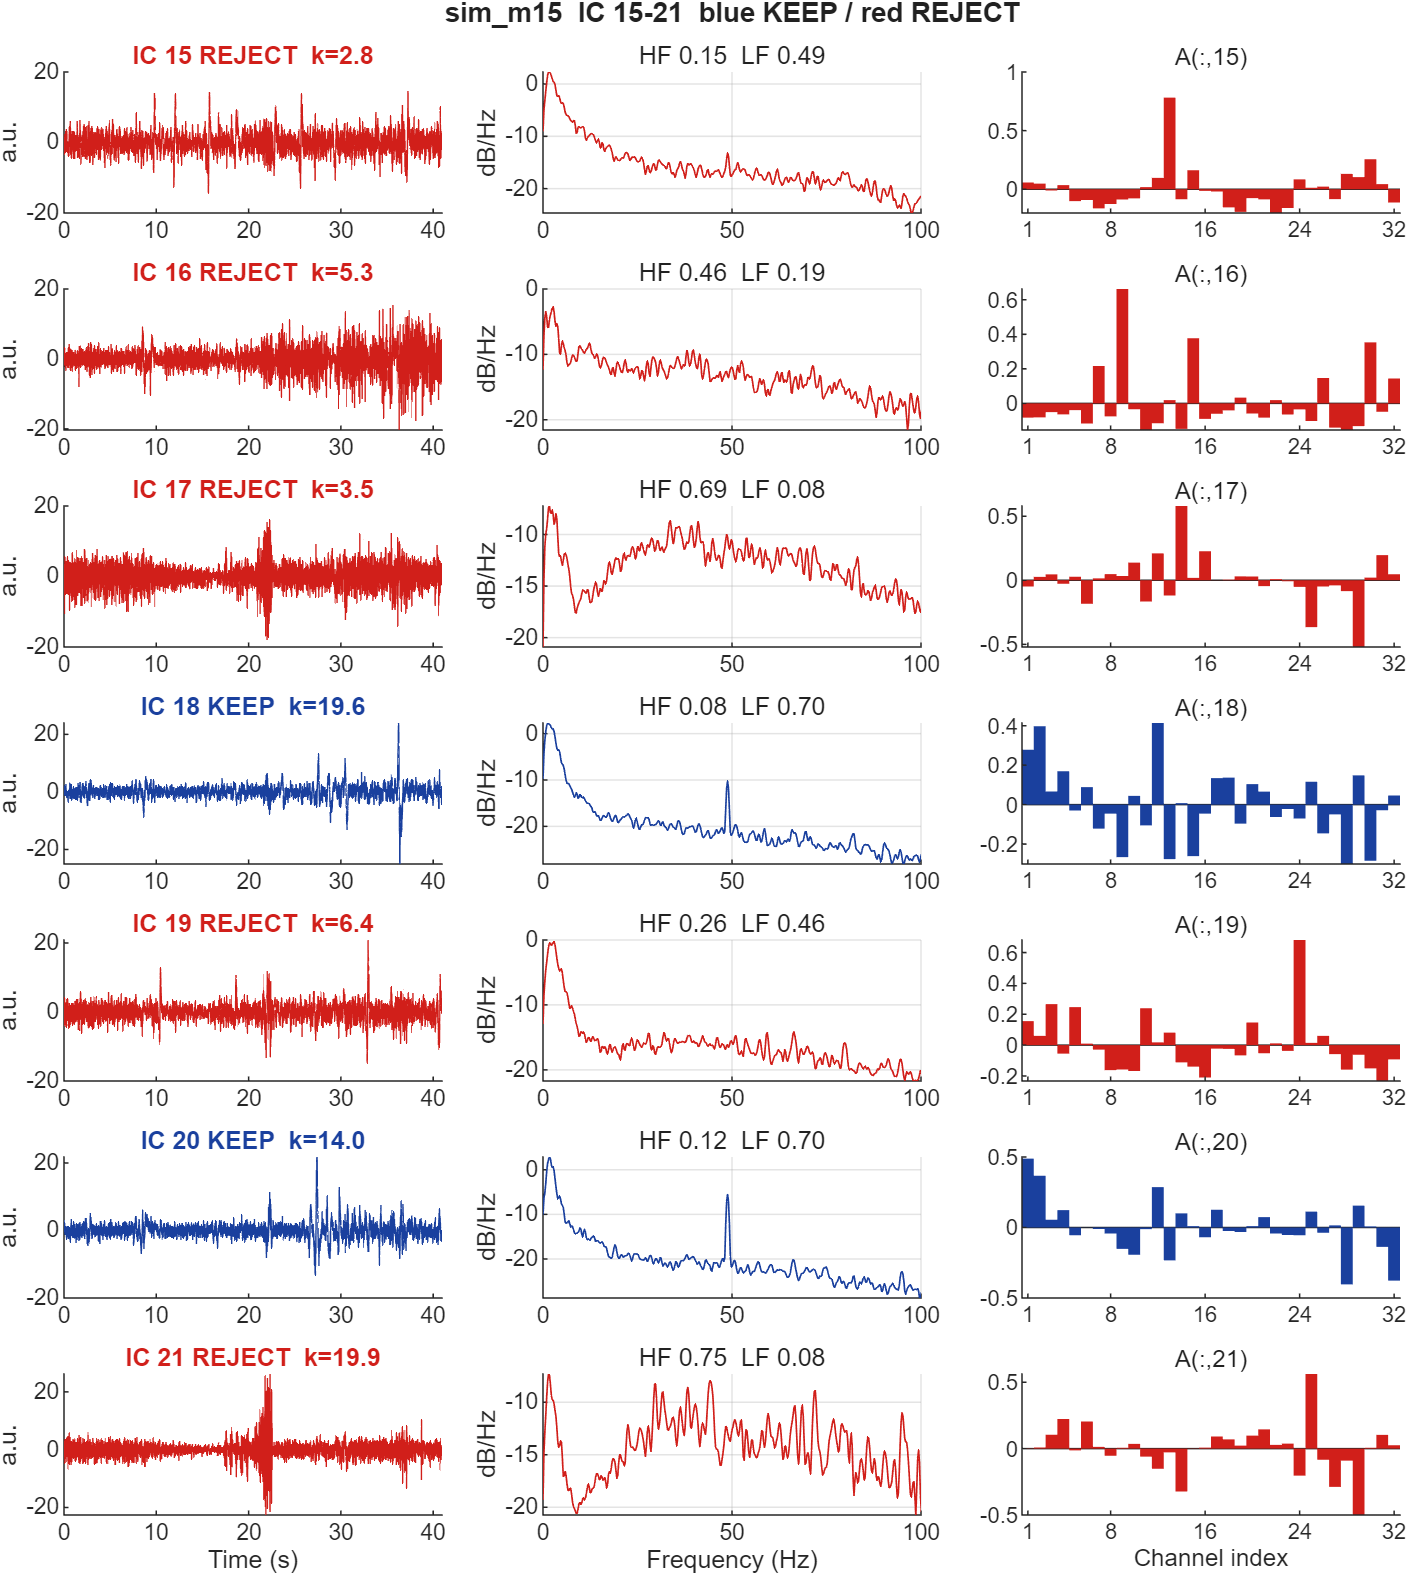
\includegraphics[height=0.80\textheight,width=0.95\textwidth,keepaspectratio]{fig23_sim_m15db_ic15_to_ic21.png}
\caption{Time course, PSD and mixing pattern of components components 15 to 21 in the $-15$~dB simulation.}
\label{fig:app23}
\end{figure}
\begin{figure}[p]
\centering
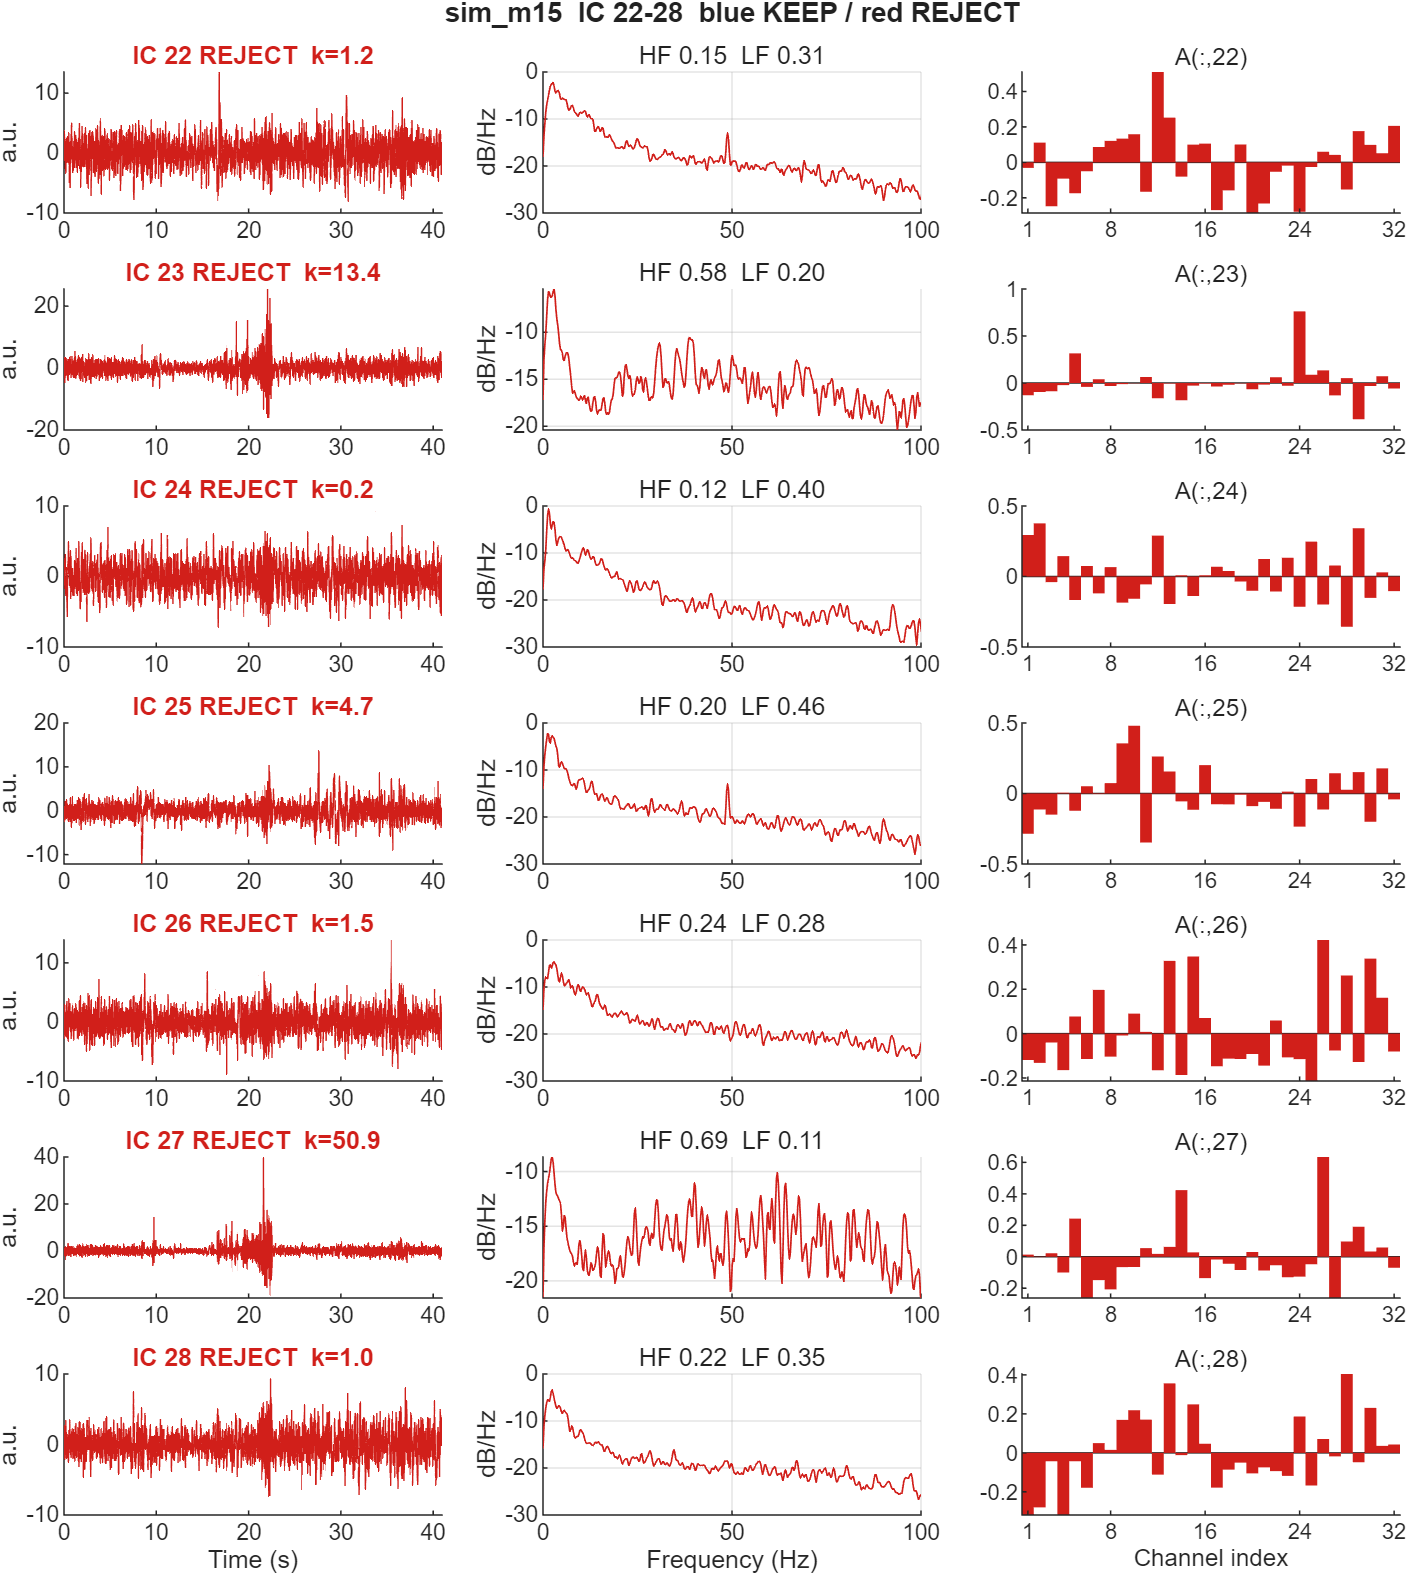
\includegraphics[height=0.80\textheight,width=0.95\textwidth,keepaspectratio]{fig24_sim_m15db_ic22_to_ic28.png}
\caption{Time course, PSD and mixing pattern of components components 22 to 28 in the $-15$~dB simulation.}
\label{fig:app24}
\end{figure}
\begin{figure}[p]
\centering
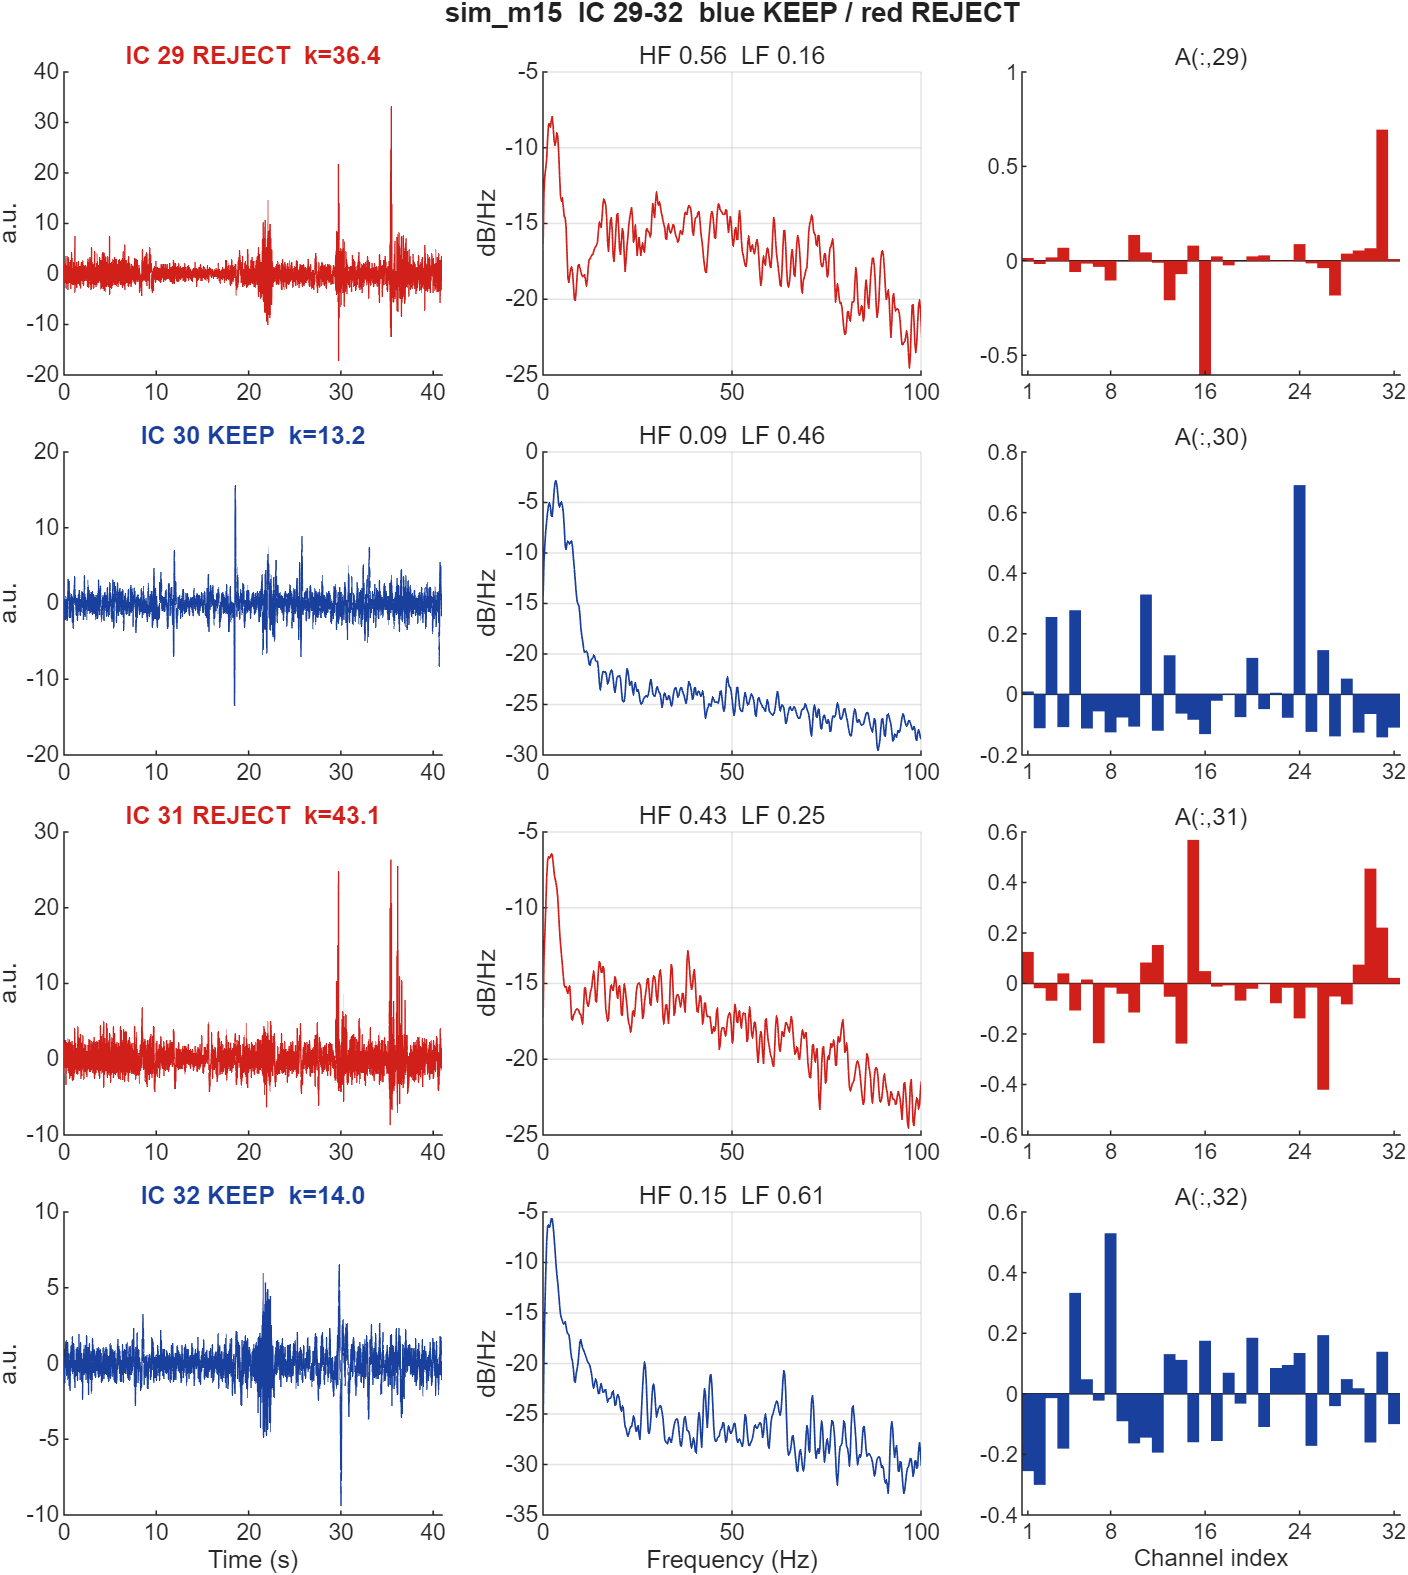
\includegraphics[height=0.80\textheight,width=0.95\textwidth,keepaspectratio]{fig25_sim_m15db_ic29_to_ic32.png}
\caption{Time course, PSD and mixing pattern of components components 29 to 32 in the $-15$~dB simulation.}
\label{fig:app25}
\end{figure}
\begin{figure}[p]
\centering
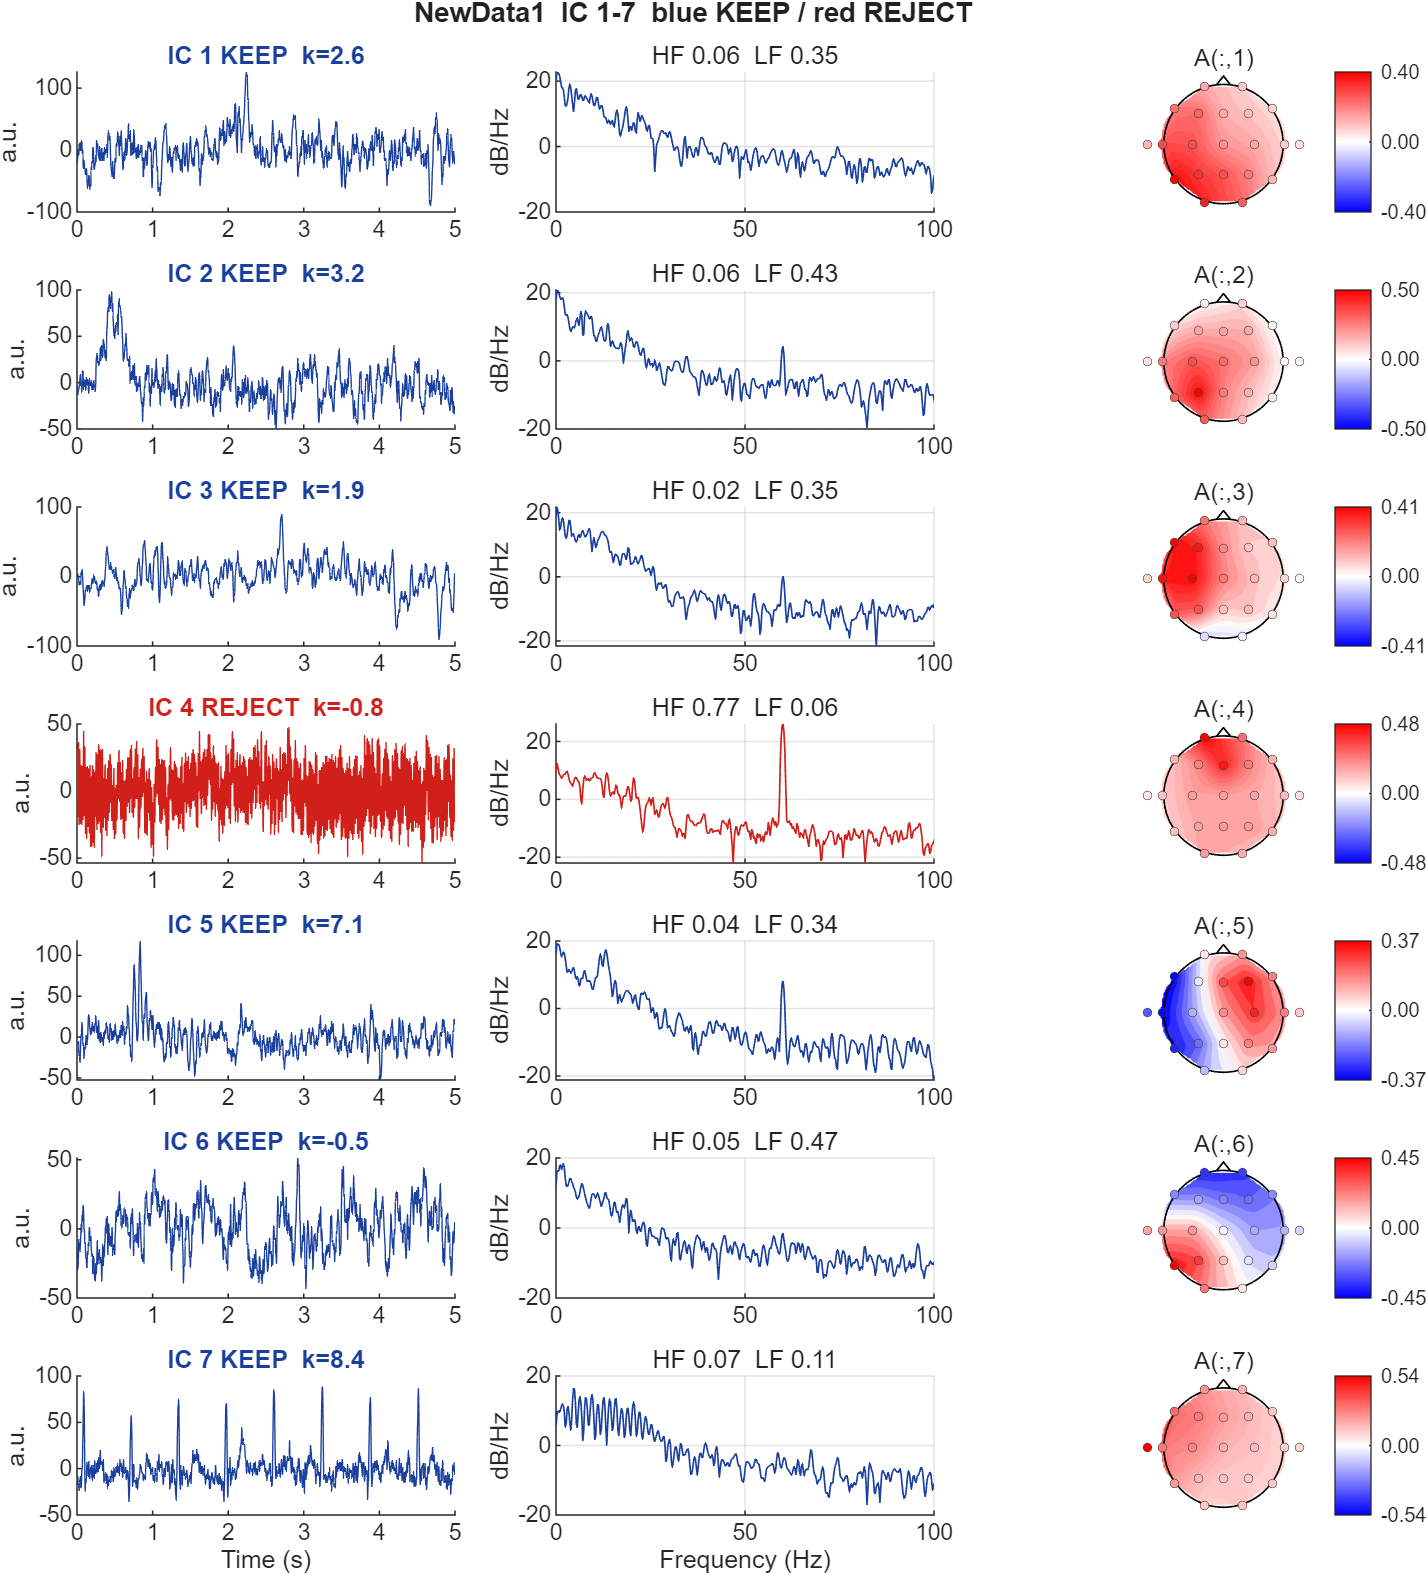
\includegraphics[height=0.80\textheight,width=0.95\textwidth,keepaspectratio]{fig26_newdata1_ic01_to_ic07.png}
\caption{Time course, PSD and mixing pattern of components components 1 to 7 in the real recording NewData1.}
\label{fig:app26}
\end{figure}
\begin{figure}[p]
\centering
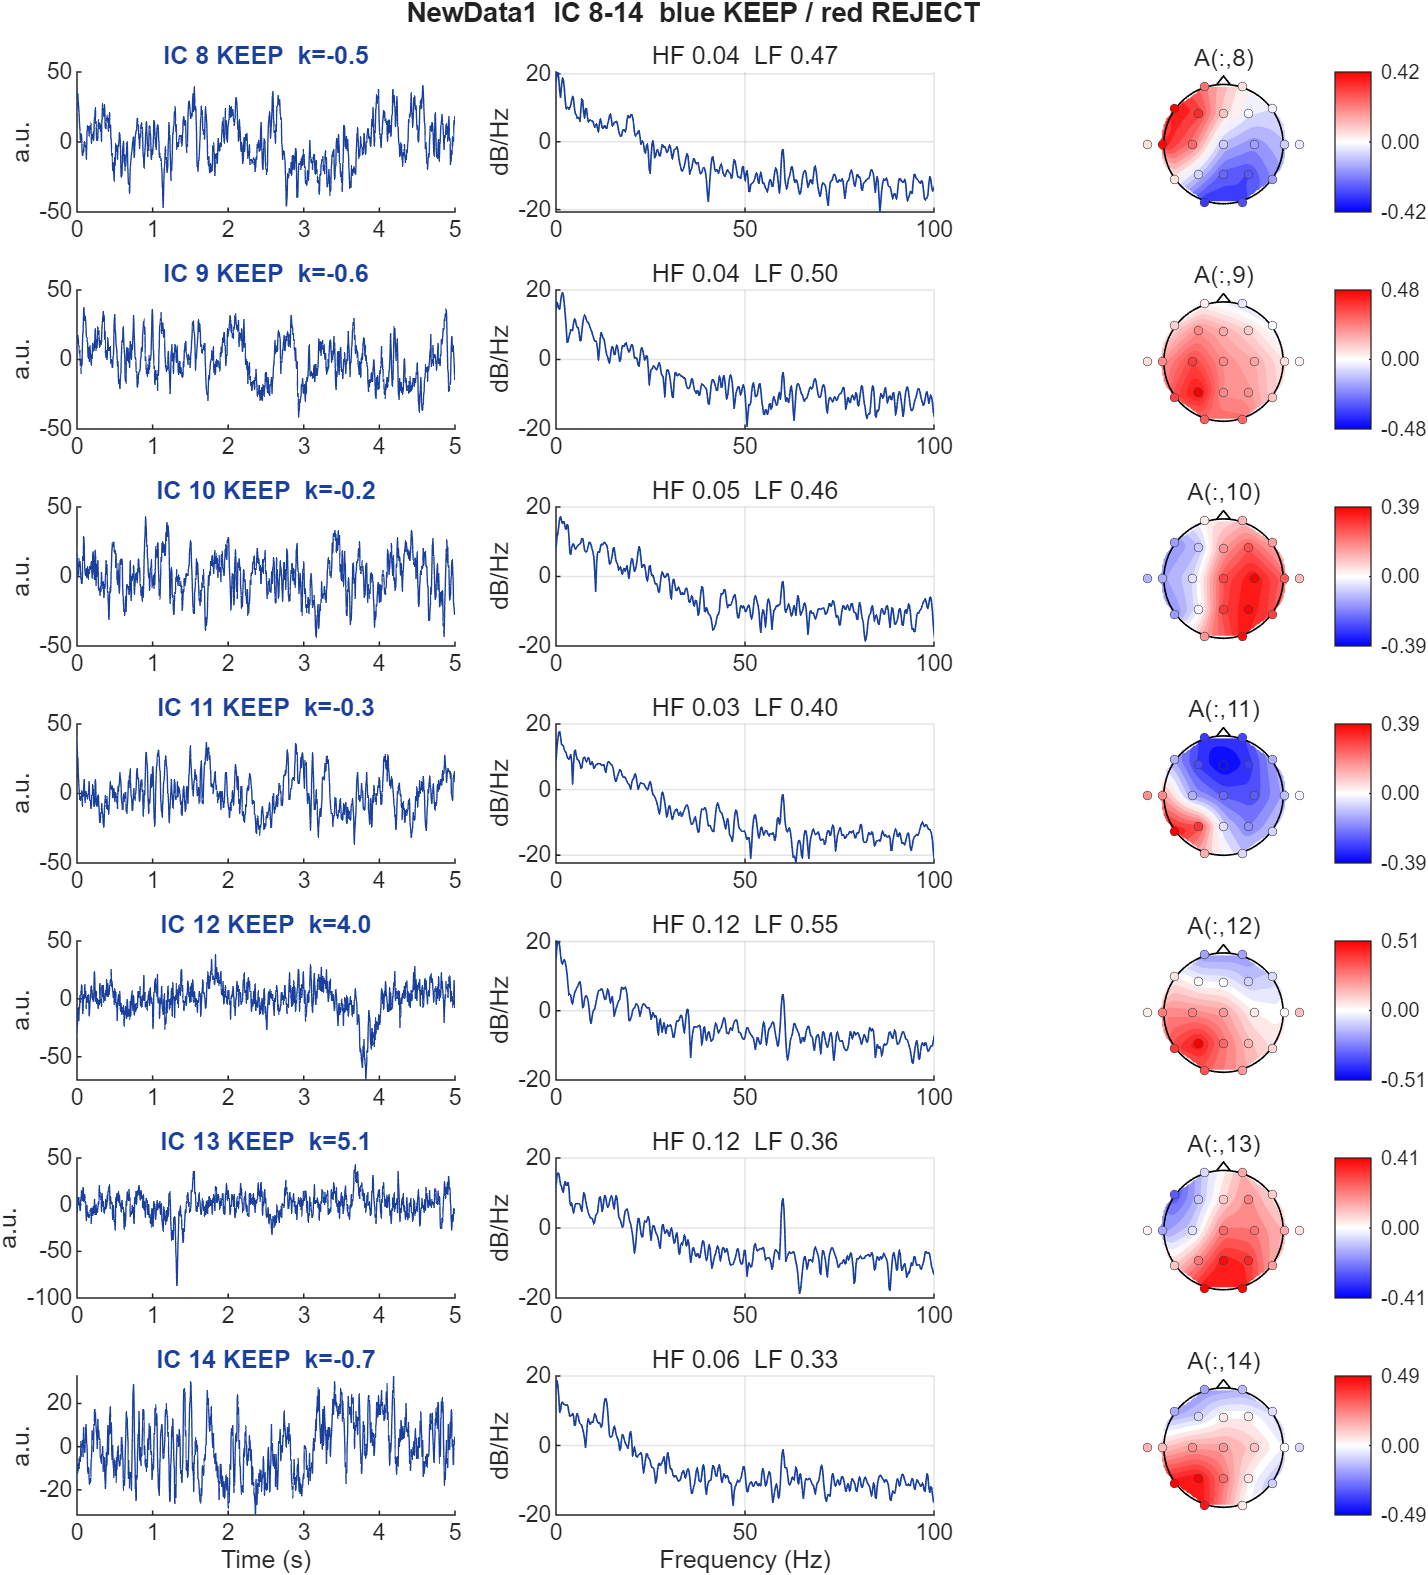
\includegraphics[height=0.80\textheight,width=0.95\textwidth,keepaspectratio]{fig27_newdata1_ic08_to_ic14.png}
\caption{Time course, PSD and mixing pattern of components components 8 to 14 in the real recording NewData1.}
\label{fig:app27}
\end{figure}
\begin{figure}[p]
\centering
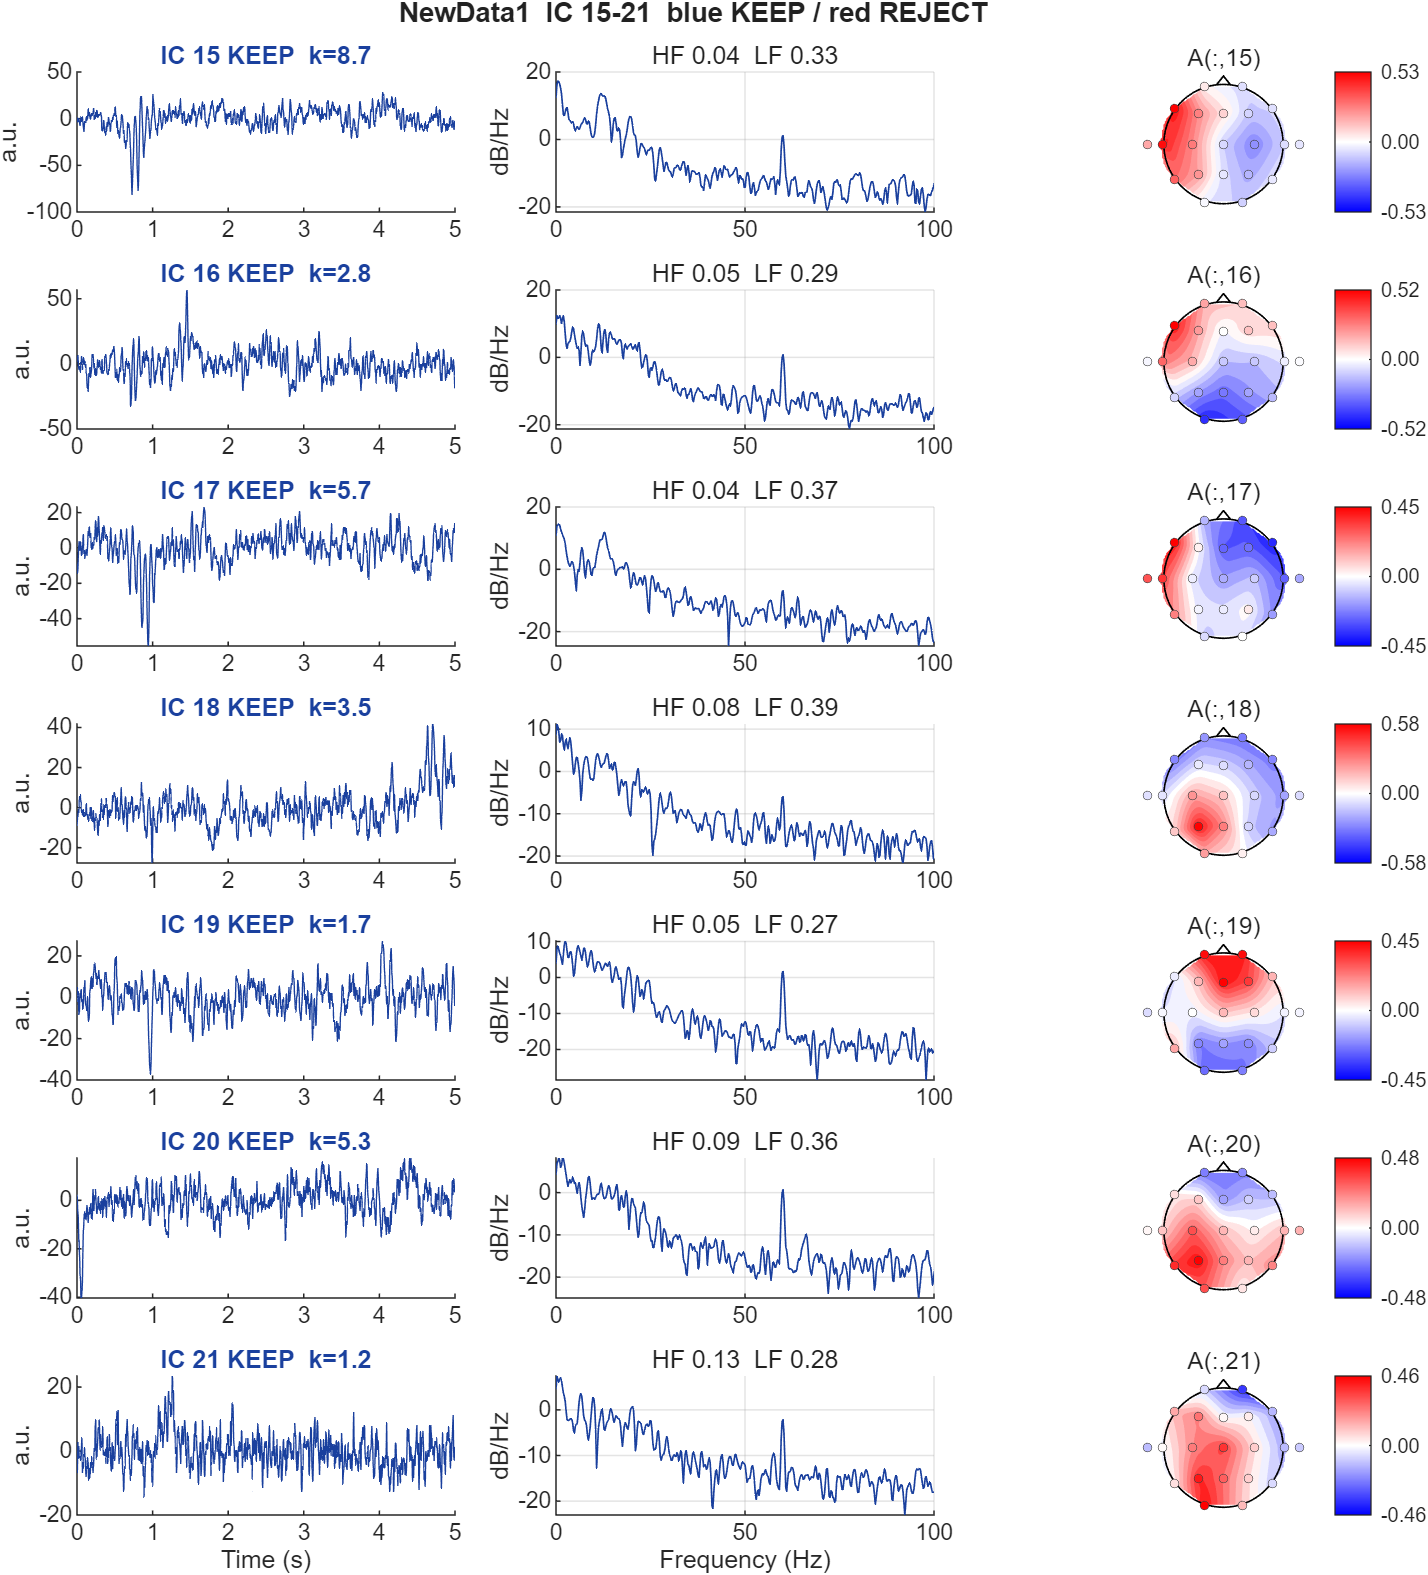
\includegraphics[height=0.80\textheight,width=0.95\textwidth,keepaspectratio]{fig28_newdata1_ic15_to_ic21.png}
\caption{Time course, PSD and mixing pattern of components components 15 to 21 in the real recording NewData1.}
\label{fig:app28}
\end{figure}
\begin{figure}[p]
\centering
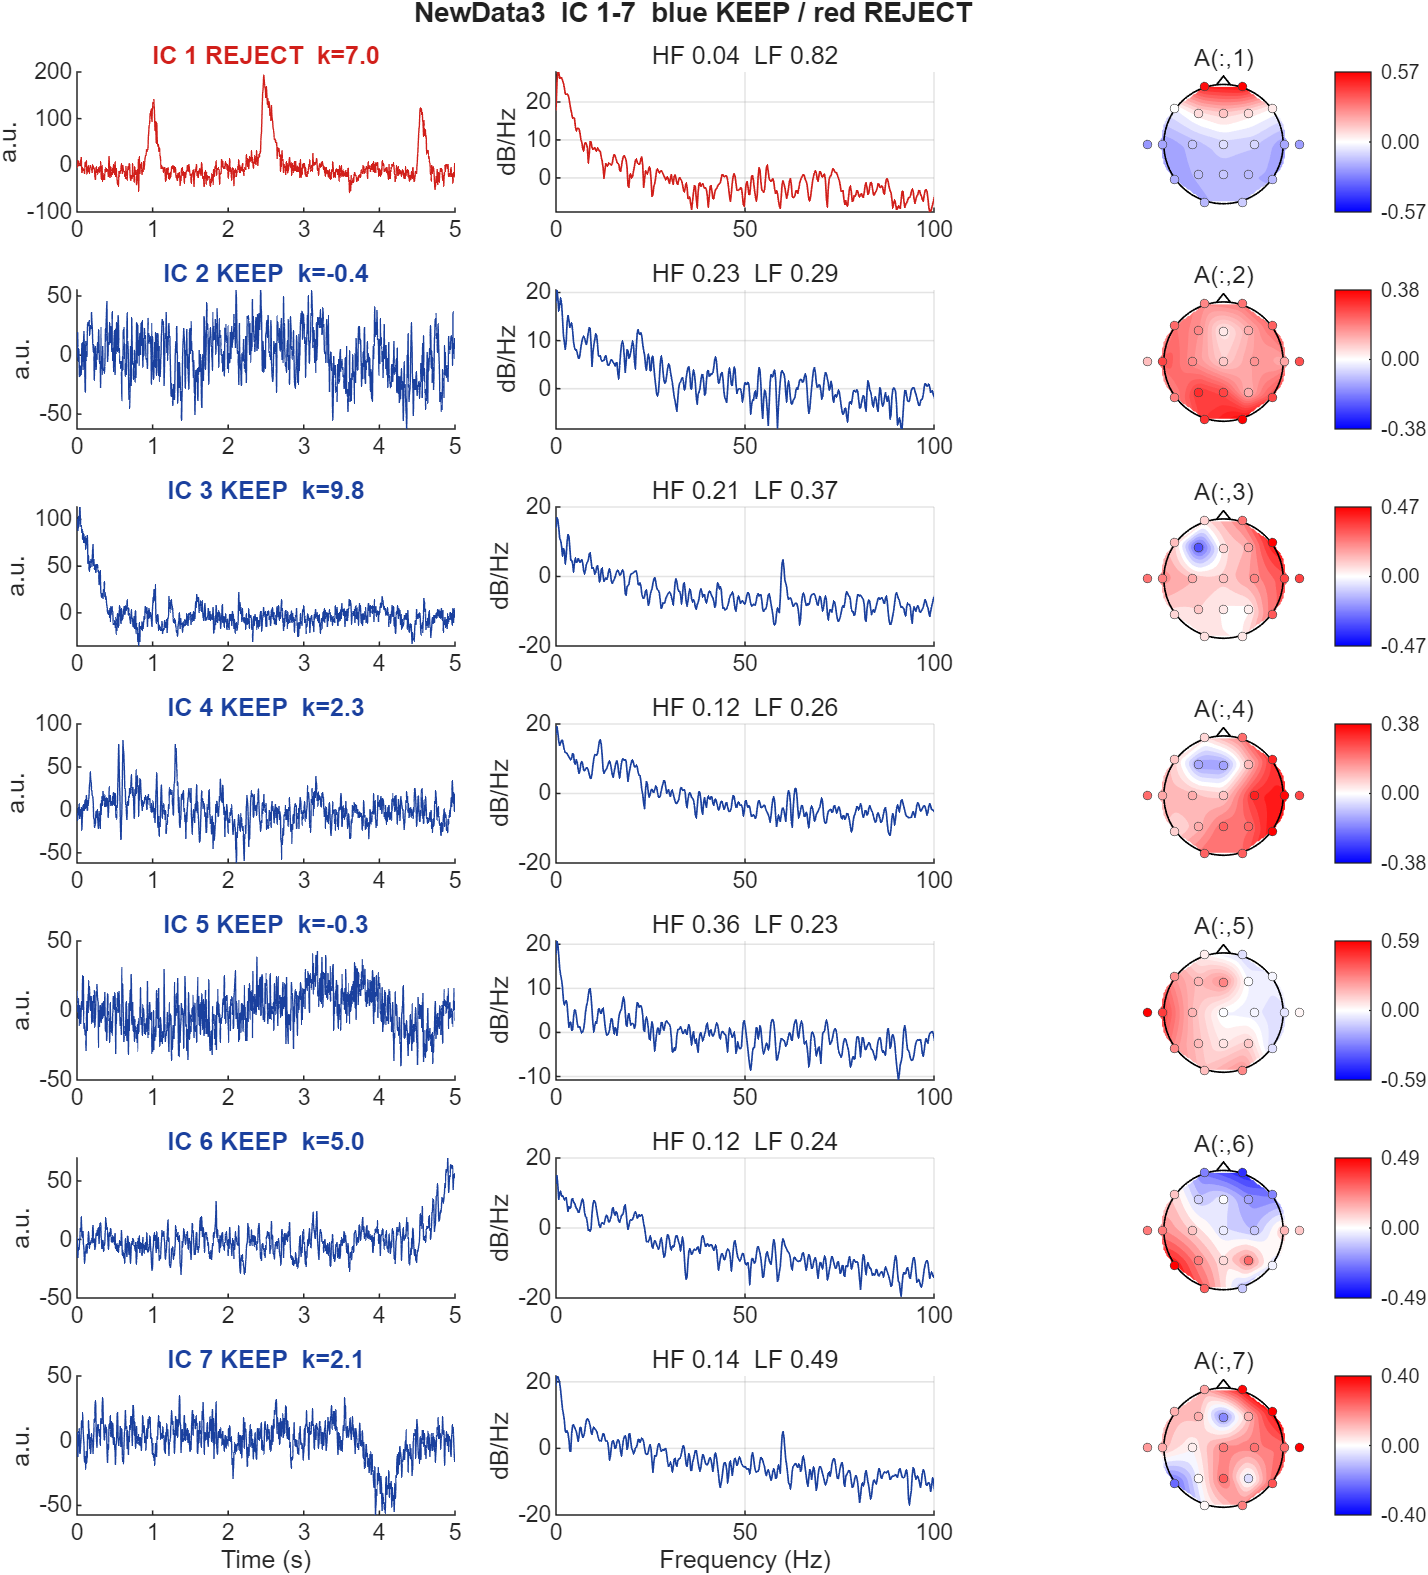
\includegraphics[height=0.80\textheight,width=0.95\textwidth,keepaspectratio]{fig29_newdata3_ic01_to_ic07.png}
\caption{Time course, PSD and mixing pattern of components components 1 to 7 in the real recording NewData3.}
\label{fig:app29}
\end{figure}
\begin{figure}[p]
\centering
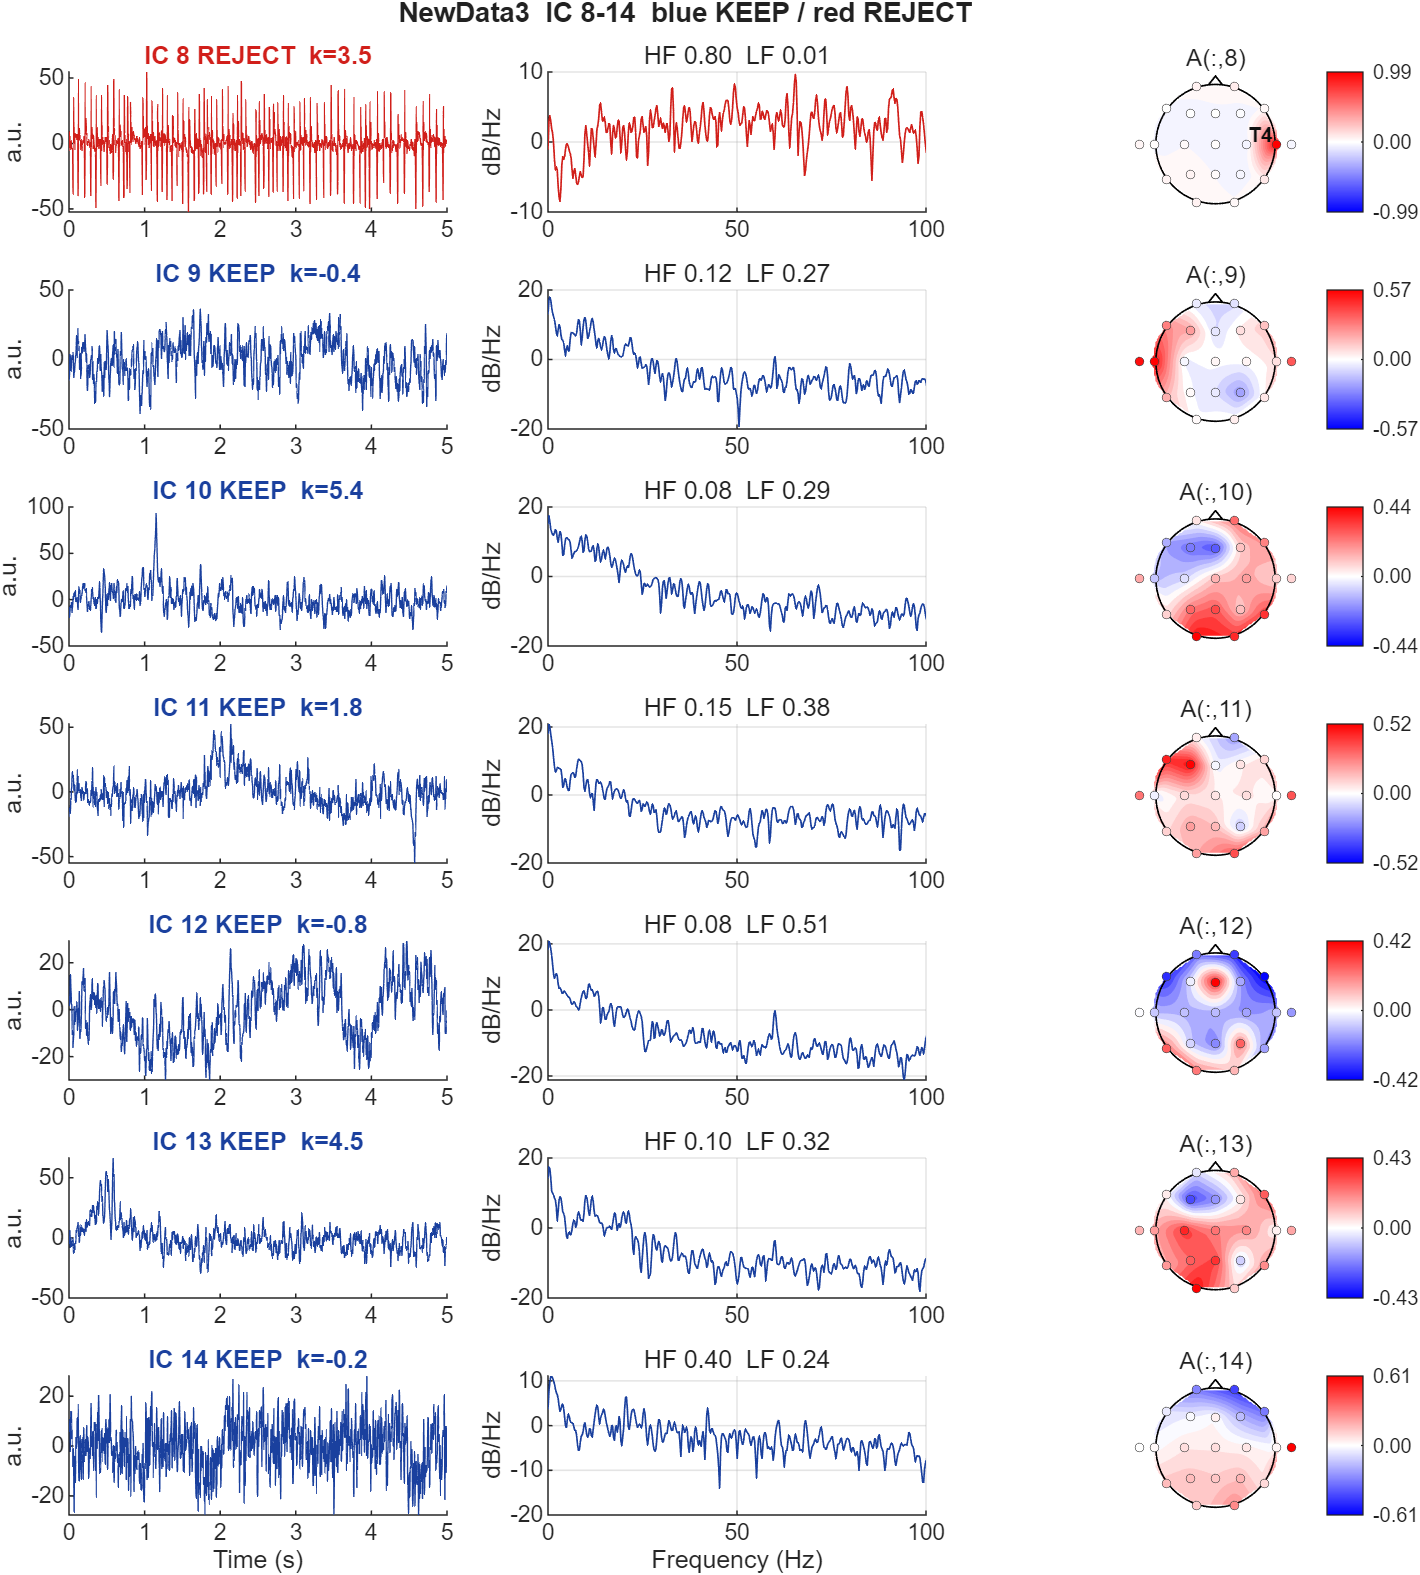
\includegraphics[height=0.80\textheight,width=0.95\textwidth,keepaspectratio]{fig30_newdata3_ic08_to_ic14.png}
\caption{Time course, PSD and mixing pattern of components components 8 to 14 in the real recording NewData3.}
\label{fig:app30}
\end{figure}
\begin{figure}[p]
\centering
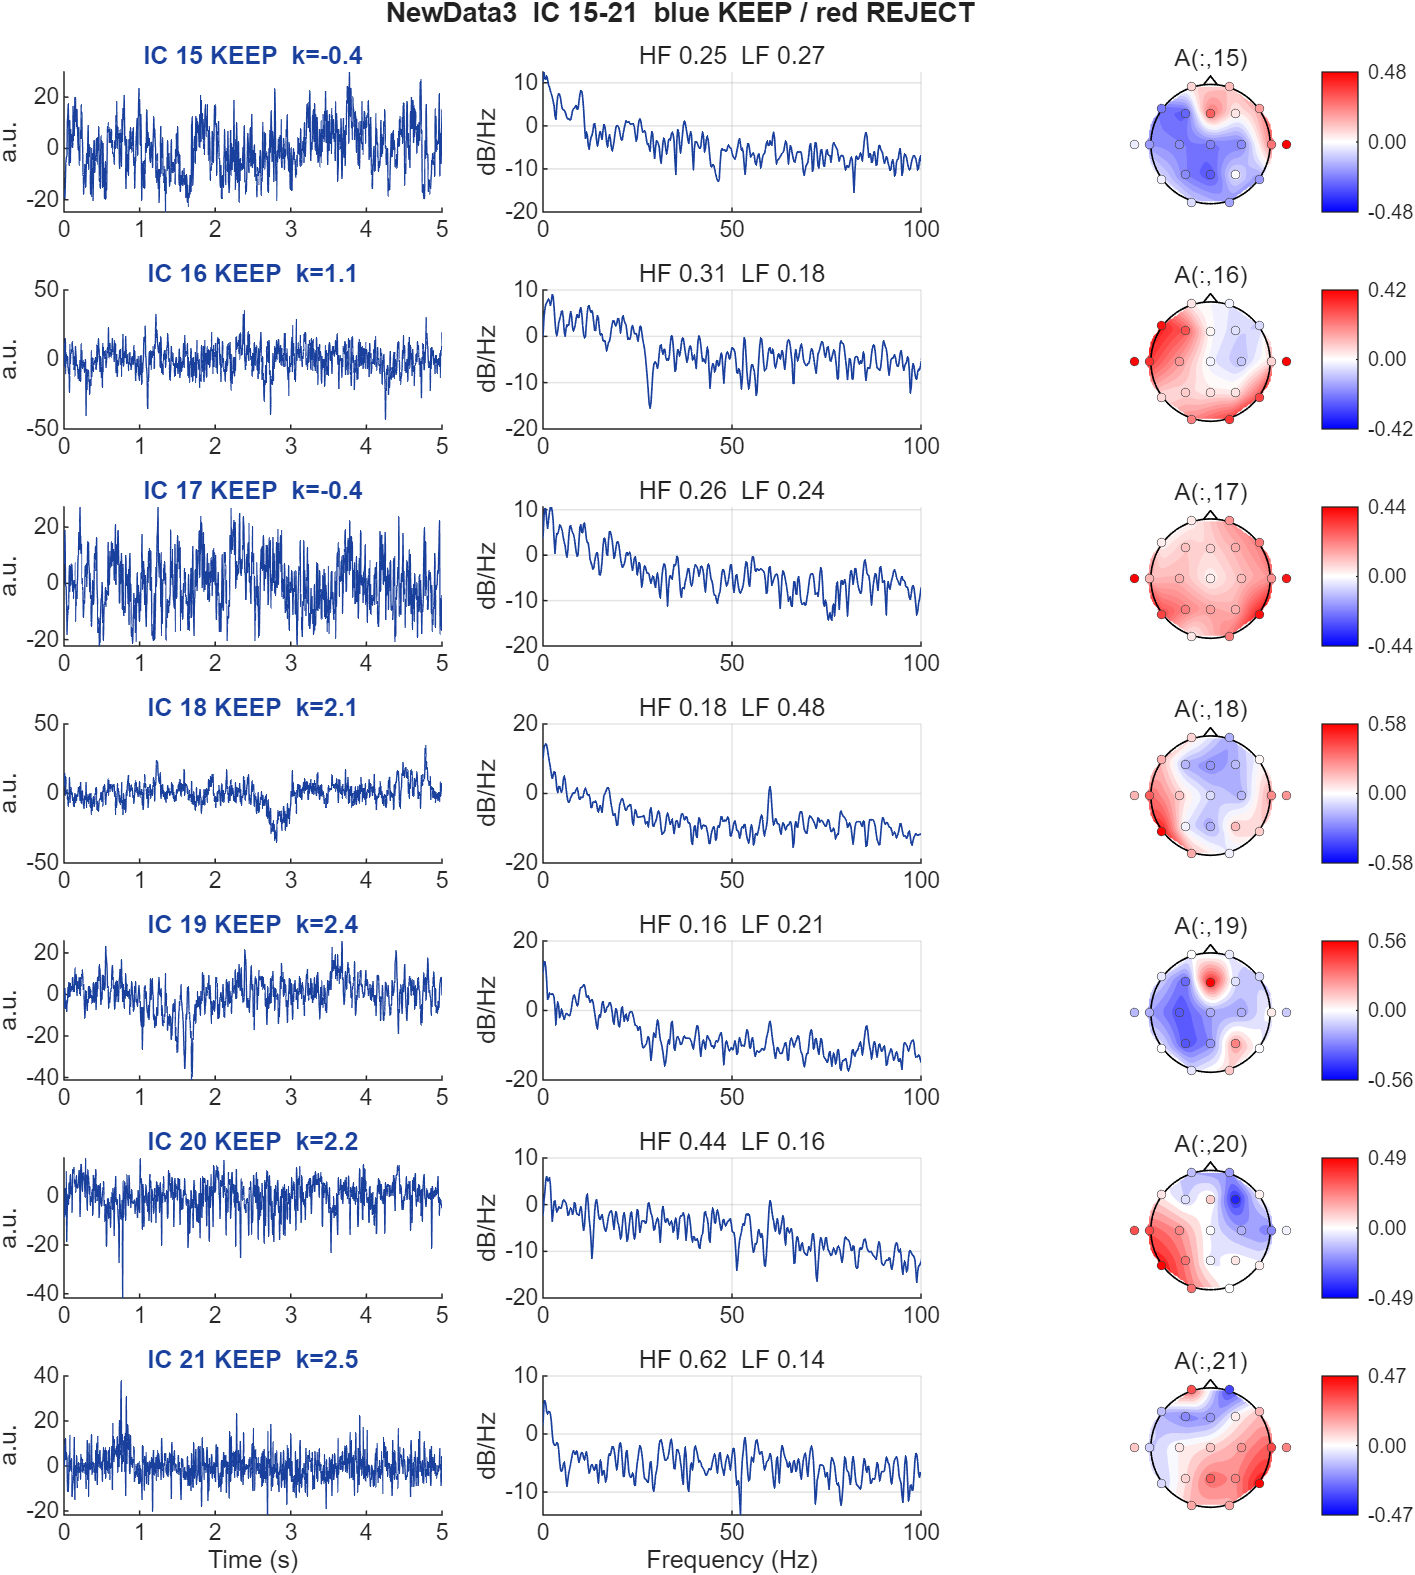
\includegraphics[height=0.80\textheight,width=0.95\textwidth,keepaspectratio]{fig31_newdata3_ic15_to_ic21.png}
\caption{Time course, PSD and mixing pattern of components components 15 to 21 in the real recording NewData3.}
\label{fig:app31}
\end{figure}
